%==============================================================================================================================================
%==============================================================================================================================================

\chapter{A P-spline Model for the Cholesky Decomposition} \label{psplines-chapter}

%\subsubsection{A tensor product P-spline model for the generalized autoregressive coefficients}


In this chapter, we demonstrate multidimensional smoothing with penalized B-splines, or \textit{P-splines}, as a flexible and computationally convenient alternative to the Hilbert space methods presented in Chapter~\ref{SSANOVA-chapter}. P-spline models are an extension of (generalized) linear regression models. They exploit the attractive properties of the B-spline basis along with the use of computationally convenient difference penalties. The formulation of the penalty is independent of the basis, which provides added modeling flexibility due to the ease with which one can employ various types of regularization. The B-spline functions have compact support, making them more attractive than the smoothing spline basis when the function to be estimated exhibits compact support as well, such as covariance matrices having banded Cholesky factor. Despite their flexibility, fitting P-spline models are only as computationally intensive as in regression modeling.  

\section{Tensor Product B-splines for Multidimensional Smoothing}

Splines are piecewise polynomial functions, where the piecewise polynomials are joined at certain values of the domain called knots. B-splines are a basis for splines. Given a set of knots, B-splines can be easily computed recursively for any polynomial degree (see \cite{de1978practical} and \cite{dierckx1995curve}). The smoothness of a fitted curve can be controlled by the number of B-splines used in the basis expansion used to approximate the curve. Fewer knots (thus, fewer basis functions) lead to smoother fits, and there is an extensive body of research focused on the choice of knot placement. Some authors have proposed adaptive smoothing techniques which attempt to automatically optimize the number and the positions of the knots; see \cite{friedman1989flexible}, \cite{kooperberg1991study}. However, this problem is nontrivial and requires nonlinear optimization, and is still an open problem today. However, limiting the number of B-splines is not the only approach to controlling the complexity of the fitted function.

\bigskip

Instead, \cite{eilers1996flexible} propose alternative an approach to nonparametric smoothing based on finite difference penalties. The difference penalties are trivial to compute and can be done so independently of the basis, unlike the smoothing spline penalty functional \eqref{eq:SS-penalty-functional}. Their approach circumvents the choice of knot specification. They achieve smoothness in fitted functions by purposefully overfitting the smooth coefficient vectors using a B-spline basis with a large number of equally spaced knots.  Augmenting the log likelihood with the difference penalty prevents overfitting and accommodates a potentially ill-conditioned fitting procedure. 

\bigskip

Analogous to the smoothing spline representation \eqref{eq:form-of-the-minimizer-phi}, we can represent $\phi$ using a B-spline basis. But first, in order to illustrate the ideas in the sections to follow, it is pragmatic to first review some basic properties of B-splines. For an exhaustive and more formal mathematical review, see  \cite{de1978practical} and \cite{dierckx1995curve}. A B-spline is a function constructed from piecewise polynomial functions which are connected in a very particular way. Their values can be computed recursively; for a non-decreasing sequence of knots $\left\{t_i\right\}$, the value of the $i^{th}$ B-spline of order $k$ can be defined using

\begin{align} 
\begin{split} \label{eq:bspline-recursive-relation}
B_{i1}\left(x\right) &= \left\{ \begin{array}{ll}
1, & t_i \le x < t_{i+1}\\
0, & otherwise
\end{array} \right.
\\
B_{ik}\left(x\right) &= \frac{x-t_i}{t_{i+k-1}-t_i}B_{i,k-1}\left(x\right) + \frac{t_{i+k}-x}{t_{i+k}-t_{i+1}}B_{i+1,k-1}\left(x\right). 
\end{split}
\end{align}

Figure~\ref{fig:overlapping-linear-cubic-bsplines} shows two sets of B-splines; the top facet displays linear B-splines and the bottom displays B-splines of degree 2. A single isolated B-spline is shown on the left side of the axis in each panel. In Figure~\ref{fig:overlapping-linear-bsplines}, the single B-spline of degree 1 consists of two linear pieces: one piece from $x_3$ to $x_4$, and the other from $x_4$ to $x_5$, which are the knots that define its support. In the right part of Figure~\ref{fig:overlapping-linear-bsplines}, three more B-splines of degree 1 are shown. Each one based on three knots. Comparing these with the overlapping quadratic B-splines in Figure~\ref{fig:overlapping-cubic-bsplines}, we can see that the extent to which neighboring B-splines overlap depends on the polynomial degree of the basis. 

\begin{figure}[H]
 \begin{center}
 \begin{subfigure}[t]{\textwidth}
  \centering
   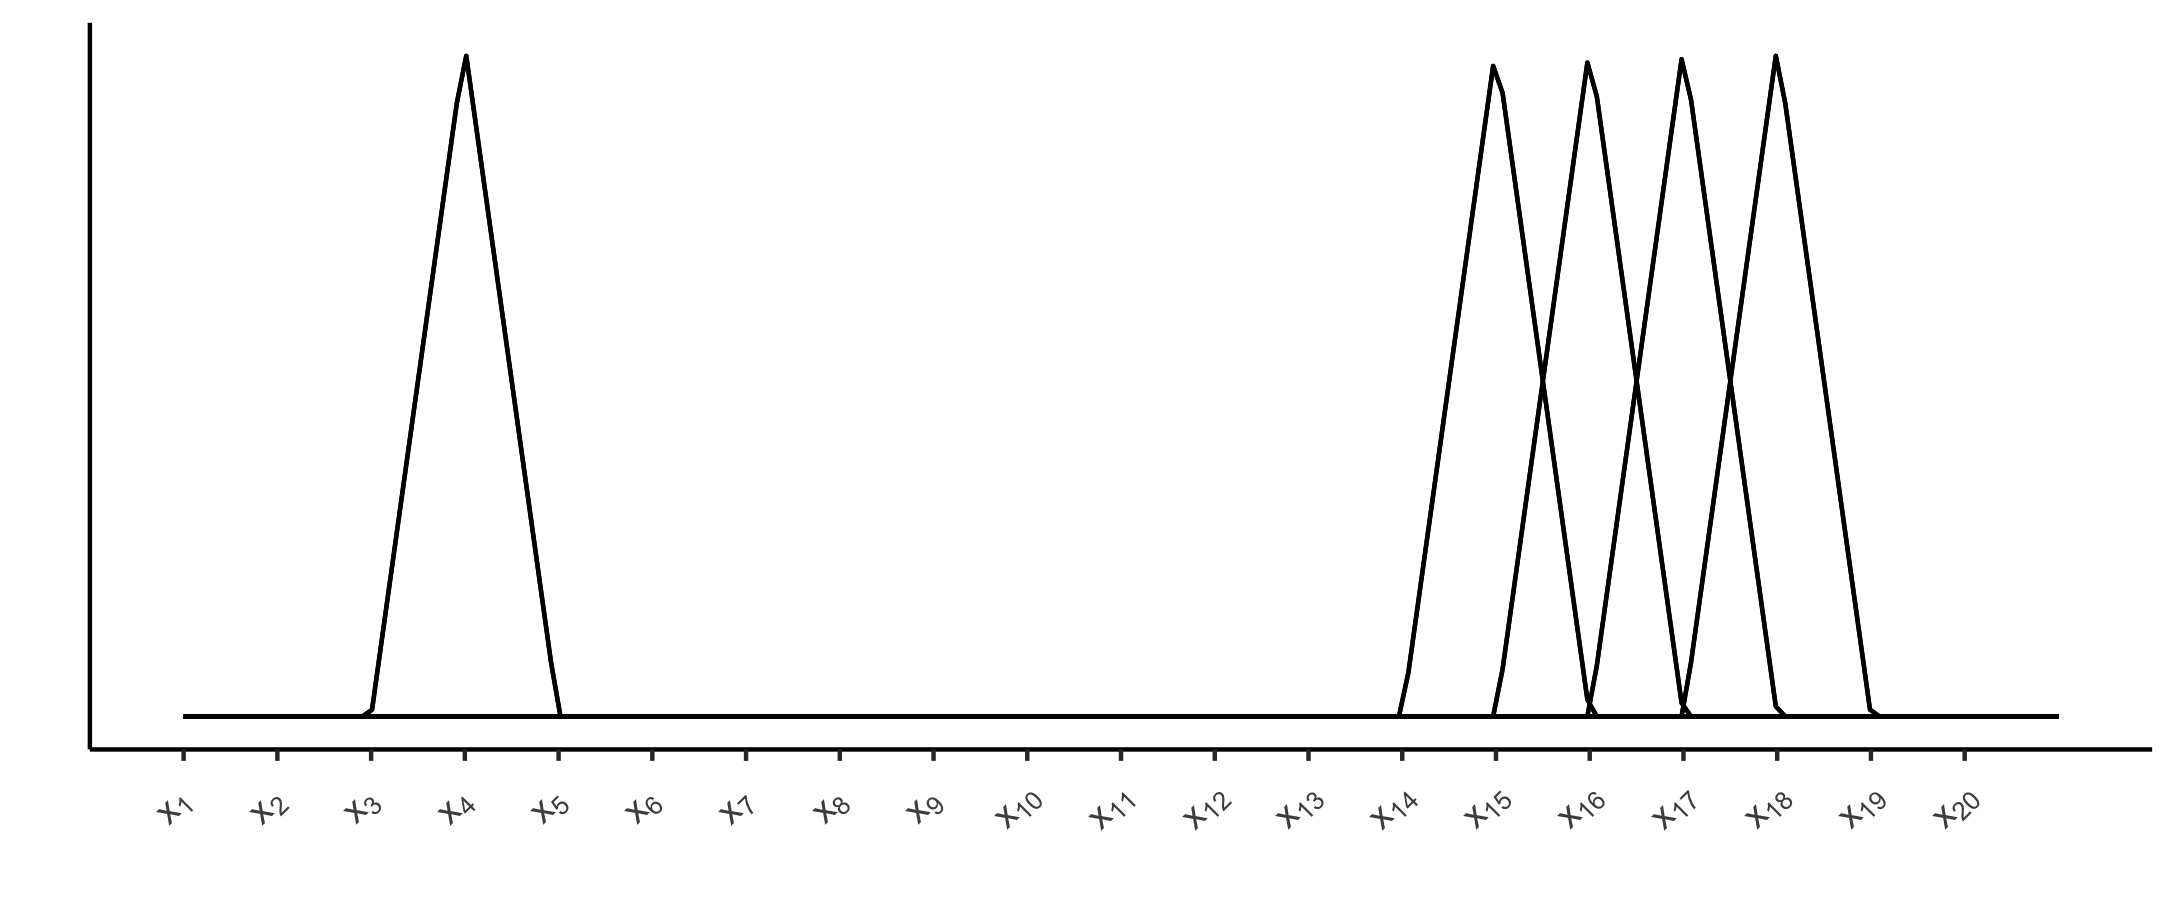
\includegraphics[width=0.75\textwidth]{img/uni_linear_bsplines}
 \caption{\textit{B-splines of degree 1} }\label{fig:overlapping-linear-bsplines}
  \end{subfigure}
   \end{center}
  \hfill
  \begin{center}
 \begin{subfigure}[t]{0.75\textwidth}
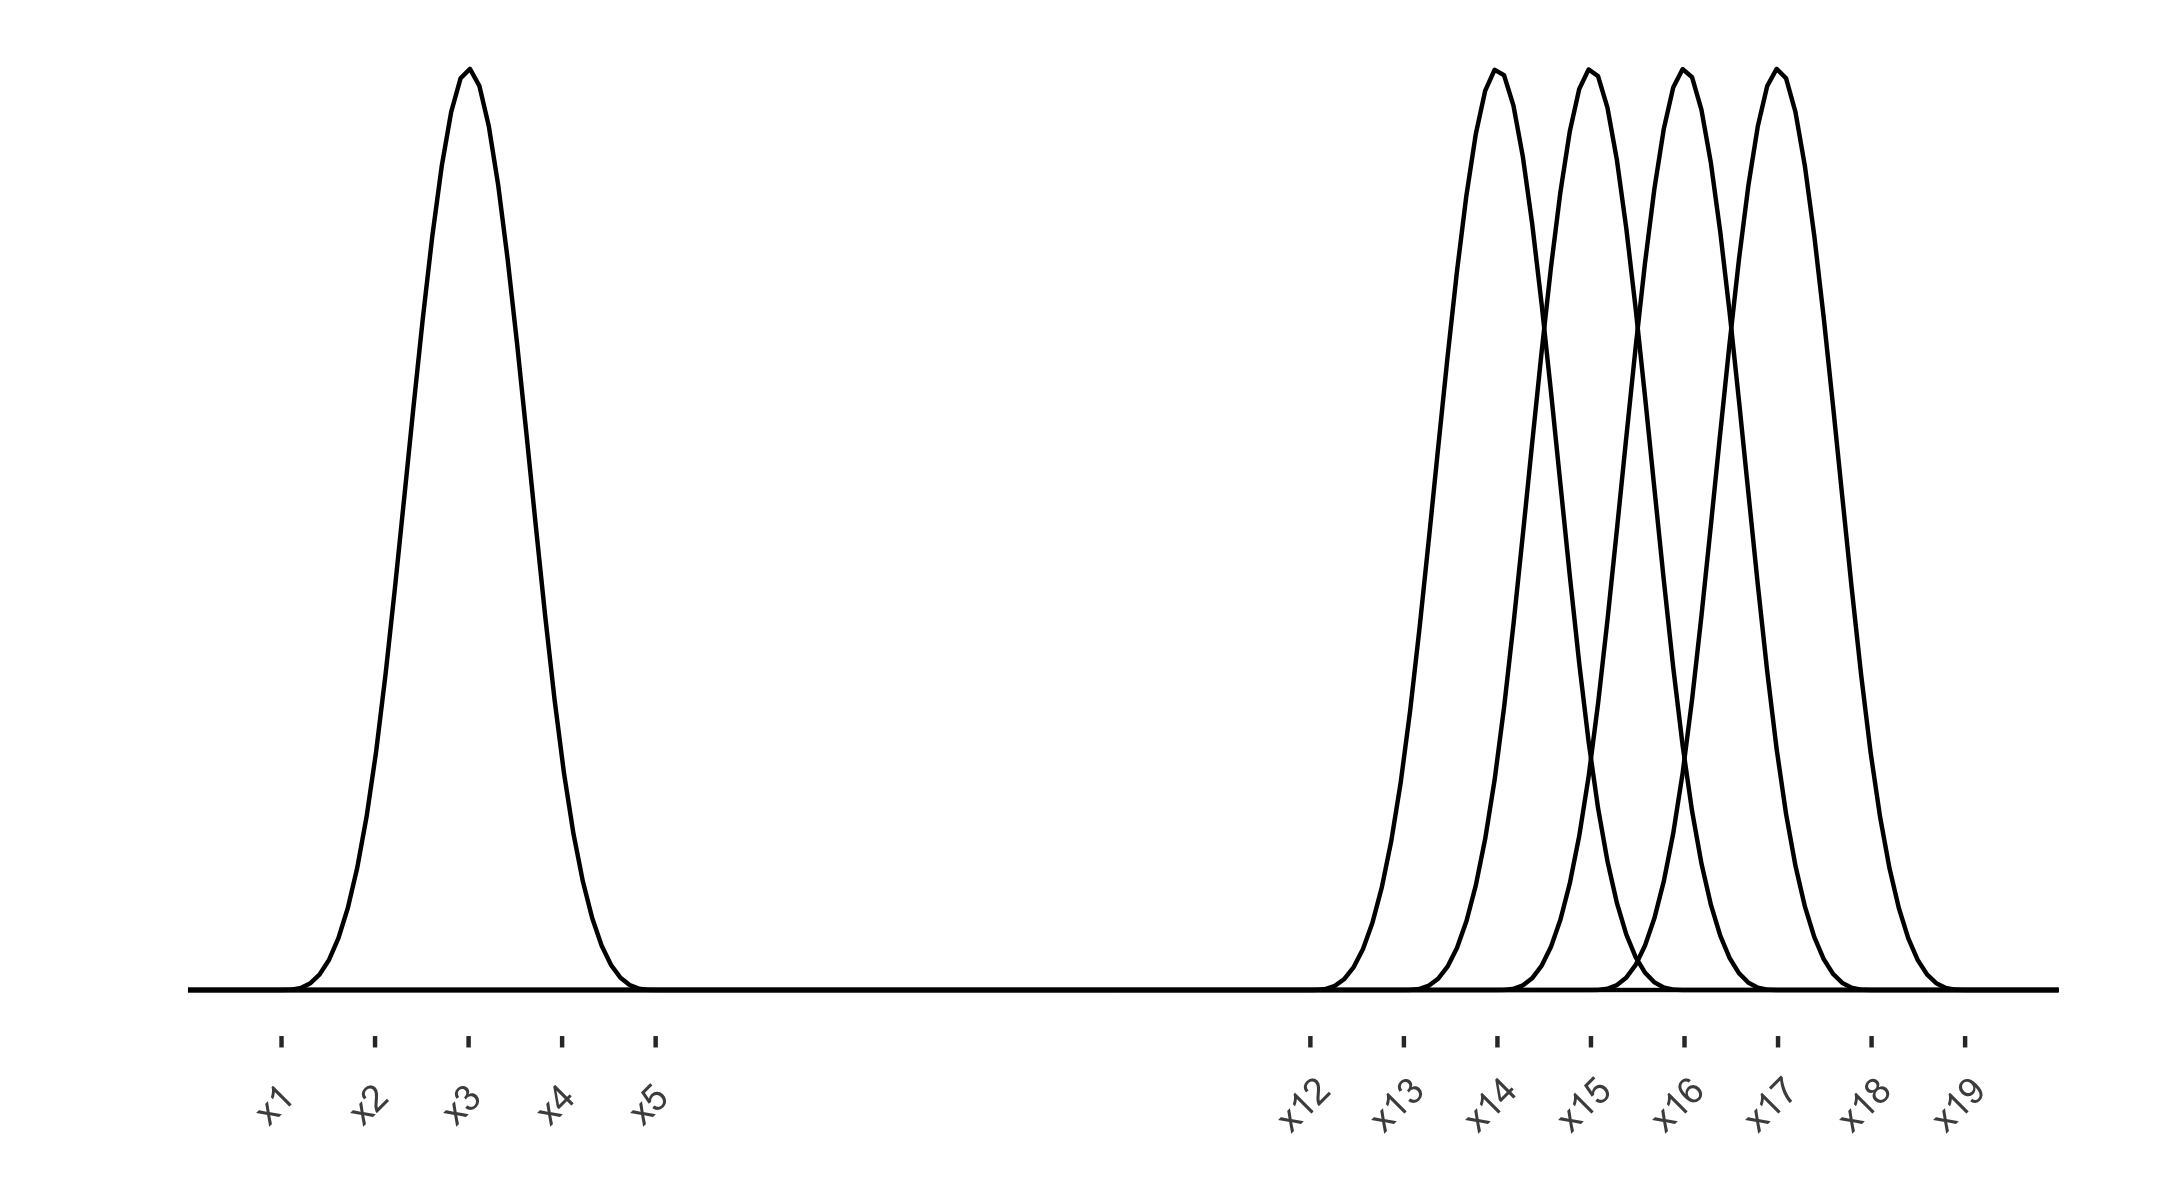
\includegraphics[width = \textwidth]{img/uni_cubic_bsplines}
 \caption{\textit{B-splines of degree 2}}
\label{fig:overlapping-cubic-bsplines}
 \end{subfigure}
 \end{center}
   \caption{\textit{ On the left: a single, isolated B-spline basis function, and on the right: several overlapping B-splines.  }}\label{fig:overlapping-linear-cubic-bsplines}
\end{figure}

B-splines make attractive basis functions for nonparametric regression; a linear combination of B-spline basis functions gives a smooth curve. Once a B-spline basis is computed, their application is no more difficult than polynomial regression, and extension to two-dimensional smoothing is available with the use of tensor products. To construct a B-spline representation for $\phi$, we need to equip the $l$ and $m$ axes each with a B-spline basis: let

\[
{B_l}_{_1}\left(l\right),\dots, {B_l}_{_{k_l}}\left(l\right)  \mbox{ and } {B_m}_{_1}\left(m\right),\dots, {B_m}_{_{k_m}}\left(m\right)
\]
\noindent
denote the B-spline bases for $l$ and $m$, each having a set of equally spaced knots along their respective domain. It is worth noting that one is free to specify a different basis for each dimension either by using different order B-spline or using different numbers of knots. Order of the basis will be indicated only when necessary and otherwise suppressed to maintain simplicity of notation. The tensor product basis functions
\begin{equation*}
T_{kk'}\left(l,m\right) = {B_l}_{_k}\left(l\right){B_m}_{_{k'}}\left(m\right)
\end{equation*}
\noindent
carve the $l$-$m$ domain into rectangles. Figure~\ref{fig:bicubic-bspline-function} shows a single $T_{kk'}$, where the marginal B-spline bases are of degree 2. For a given knot grid, we can approximate $\phi$ by
\begin{equation} \label{eq:tensor-product-bspline-expansion-phi}
\phi\left(l,m\right) = \sum_{r=1}^{k_l} \sum_{c=1}^{k_m} \theta_{rc} {B_l}_{_r}\left(l\right) {B_m}_{_c}\left(m\right). 
\end{equation}
\noindent
%Substituting this expression for $\phi$ in the negative log likelihood \eqref{eq:full-joint-likelihood} gives
%\begin{align}
%\begin{split} \label{eq:full-joint-likelihood-BS}
%-2\ell\left(\theta_{11},\dots, \theta_{k_l,k_m} \vert Y_1,\dots, Y_N, \sigma^2\right)  = \sum_{i=1}^N \sum_{j=2}^{p_i} \log\sigma_{ij}^2 +  \sum_{i=1}^N \sum_{j=2}^{p_i} \frac{1}{\sigma^{2}_{ij}}\left( y_{ij} - \sum_{k<j}\left[ \sum_{r=1}^{k_l} \sum_{c=1}^{k_m} \theta_{i'j'} {B_l}_{_{r}}\left(l_{ijk}\right) {B_m}_{_{c}}\left(m_{ijk}\right)\right] y_{ik}  \right)^2.
%\end{split}
%\end{align}
% For fixed $\sigma^2$ as in \eqref{eq:penalized-joint-loglik-given-sigma}, we define the estimator of $\phi$ as the minimizer of 
%\begin{equation} 
%-2\ell\left(\phi \vert Y_1,\dots, Y_N\right) + \lambda J_{\lambda}\left(\phi\right) = \sum_{i=1}^N \sum_{j=2}^{p_i} \sigma^{-2}_{ij}\left( y_{ij} - \sum_{k<j} \phi\left(\bfv_{ijk}\right) y_{ik}  \right)^2 + \lambda J\left( \phi \right),
%\end{equation} 
%\noindent
%where $J\left(\phi\right)$ is a penalty on the roughness of the fitted function. 
%
%
\begin{figure}[H]
    \begin{center}
 \begin{subfigure}[t]{0.48\textwidth}
  \centering
  \includegraphics[width=\textwidth]{img/bicubic_basis_function}
  \end{subfigure}
 \begin{subfigure}[t]{.48\textwidth}
  \centering
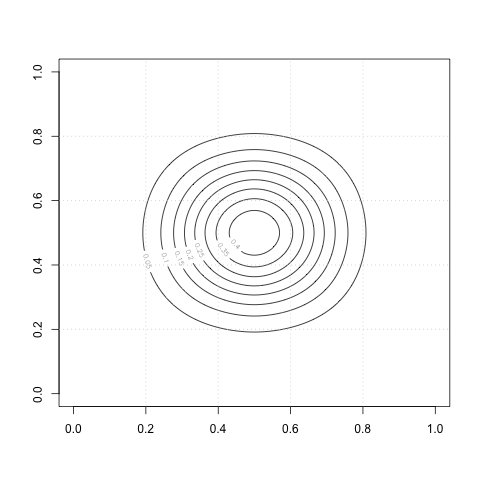
\includegraphics[width=\textwidth]{img/bicubic_bspline_contour}
 \end{subfigure}
  \caption{\textit{ Tensor product of two quadratic B-splines }}\label{fig:bicubic-bspline-function}
 \end{center}
\end{figure}

%%%%%%%%%%%%%%%%%%%%%%%%%%%%%%%%%%%%%%%%%%%%%%%%%%%%%%%%%%%%%%%%%%%%%%%%%%%%%%%%%%%%%%%%%%%
%%%%%%%%%%%%%%%%%%%%%%%%%%%%%%%%%%%%%%%%%%%%%%%%%%%%%%%%%%%%%%%%%%%%%%%%%%%%%%%%%%%%%%%%%%%
%%%%%%%%%%%%%%%%%%%%%%%%%%%%%%%%%%%%%%%%%%%%%%%%%%%%%%%%%%%%%%%%%%%%%%%%%%%%%%%%%%%%%%%%%%%
%%%%%%%%%%%%%%%%%%%%%%%%%%%%%%%%%%%%%%%%%%%%%%%%%%%%%%%%%%%%%%%%%%%%%%%%%%%%%%%%%%%%%%%%%%%

\section{Difference Penalties}

The specification of a P-spline model provides a simple way to avoid the issue of optimal knot selection for the $l$ and $m$ bases. This is done by constructing the marginal B-spline bases with a large number of knots - more than necessary. Application of a smoothness penalty prevents overfitting. A penalty based on discrete differences of the B-spline coefficients controls the fit in a way much like the classical second derivative penalty \eqref{eq:SS-penalty-functional} does. However, its construction is trivial even when the number of basis functions is very large. Using the properties of B-splines, it is straightforward to show that the difference penalty of order $d$ approximates the integrated square of the $d^{th}$ derivative well, so little is lost by using it in place of the derivative-based penalty. \cite{o1986statistical} established that for $f\left(x\right) = \sum\limits_{j=1}^k \theta_j B_j\left(x\right)$, one can derive a banded matrix $P$ using the properties of B-splines such that $J\left(f\right) = \int_0^1 \left( f^{\prime \prime}\left(x\right)\right)^2$ can be written
 \[
J\left(f\right) = \theta^\prime P \theta
 \] 
\noindent
where $\theta = \left(\theta_1,\dots, \theta_k\right)$ denotes the vector of B-spline basis coefficients. The $\left(i,j\right)$ element of the penalty matrix $P$ is given by
 \[
 p_{ij} = \int_0^1 B_i^{\prime \prime}\left(x\right) B_j^{\prime \prime}\left(x\right).
 \]
\cite{wand2008semiparametric} extend the work in \cite{o1986statistical} to higher order derivatives for general degree B-splines and derive an exact matrix algebraic expression for the penalty matrices.  The computation of $P$ is nontrivial and becomes very tedious when the third and fourth derivative are used as the roughness measure. In the cubic case, the expression is a result of the application of Simpson's Rule applied to the inter-knot differences since each $B_i^{\prime \prime} B_j^{\prime \prime}$ is a piecewise quadratic function. The penalty may be written
 \[
 P = \left(B^{\prime \prime}\right)^\prime \textup{diag}\left(\omega \right) B^{\prime \prime}, 
 \]
 \noindent
 where $B^{\prime \prime}$ is the $3\left( k + 7 \right) \times \left( k + 4 \right)$ matrix with $i$-$j^{th}$ entry given by $B_j^{\prime \prime} \left(x_i^*\right)$, $x^*_i$ is the $i^{th}$ element of 
\[
\left( \theta_1,\frac{\theta_1+\theta_2}{2},\theta_2,\theta_2,\frac{\theta_2+\theta_3}{2},\theta_3,\dots,\theta_{k+7},\frac{\theta_{k+7}+\theta_{k+8}}{2},\theta_{k+8} \right),
\]
 \noindent
 and $\omega$ is the $3\left(k+7\right) \times 1$ vector given by
\begin{align*}
\omega &= \left( \frac{1}{6}\left(\Delta \theta \right)_1,\frac{4}{6}\left(\Delta \theta \right)_1, \frac{1}{6}\left(\Delta \theta \right)_1,\frac{1}{6}\left(\Delta \theta \right)_2, \frac{4}{6}\left(\Delta \theta \right)_2,  \right. \\
&\qquad   \left. {} \frac{1}{6}\left(\Delta \theta \right)_2 , \dots , \frac{1}{6}\left(\Delta \theta \right)_{n+7}, \frac{4}{6}\left(\Delta \theta \right)_{k+7}, \frac{1}{6}\left(\Delta \theta \right)_{k+7}  \right) \\
\end{align*}
\noindent
where $\left(\Delta \theta \right)_j = \theta_{j+1}-\theta_j$. They generalize this to the case of any order penalty and present a table of formulas for constructing any arbitrary penalty matrix, $P$.  

\bigskip

Alternatively, \cite{eilers1996flexible} replace the curvature penalty \eqref{eq:SS-penalty-functional} with a finite difference penalty on the B-spline coefficients. They suggest enforcing smoothness of fitted functions $f\left(x\right) = \sum\limits_{j=1}^k \theta_i B_j\left(x\right)$ using the $d^{th}$ order difference penalty:
\begin{equation} \label{eq:bspline-difference-penalty-1}
J_d\left( f \right) = \sum_{j=d}^k \left(\Delta^d \theta_j\right)^2.
\end{equation} 
\noindent
where $\Delta \theta_j = \theta_j - \theta_{j-1}$, and $\Delta^2 \theta_j = \Delta\left(\Delta \theta_j\right) = \theta_j - 2\theta_{j-1} + \theta_{j-2}$. In general, $\Delta^d \theta_j = \Delta\left(\Delta^{d-1} \theta_j \right)$. Let $D_d$ denote the differencing operator:
\[
D_d\theta = \Delta^d \theta.
\]
\noindent
Then, \eqref{eq:bspline-difference-penalty-1} can be written in terms of the squared norm of the difference operator applied to the vector of B-spline coefficients:
\begin{align} 
\begin{split} \label{eq:bspline-difference-penalty-2}
J_d\left( f \right) &= \vert \vert D_d\theta \vert \vert^2 \\
&= \theta^\prime P_d \theta
\end{split}
\end{align}
\noindent
where $P_d = D_d^\prime D_d$.  The connection between the second-derivative penalty to the penalty on second-order differences of the B-spline coefficients can be established with straightforward calculus and the recursive property of the B-spline basis functions.  The derivative properties of B-splines permits the traditional smoothness penalty applied to $f$ to be written 
%\begin{equation*} 
%\int_0^1 \left( f^{\prime \prime}\left(x\right)\right)^2\;dx = \int_{0}^{1} \left\{ \sum\limits_{j=1}^k  \theta_j B_{j3}^{\prime \prime}\left(x\right) \right\}^2\; dx.
%\end{equation*}
%\noindent
\begin{equation*} \label{eq:second-derivative-bspline-penalty}
\int_0^1 \left( f^{\prime \prime}\left(x\right)\right)^2\;dx =  \int_{0}^{1}  \bigg[ \sum\limits_{i=1}^k \sum\limits_{j=1}^k \Delta^2 \theta_i \Delta^2 \theta_j B_{i,1}\left(x\right)B_{j,1}\left(x\right) \;dx\bigg]. 
\end{equation*}
\noindent
where $B_{j,1}\left(x\right)$ is the $j^{th}$ B-spline of order 1. Most of the cross products of $B_{i,1}$ and $B_{j,1}$ vanish since B-splines of degree 1 only overlap when $j$ is $i-1$, $i$, or $i+1$. Thus, we have that
\begin{align}
\begin{split}
\int_0^1 \left( f^{\prime \prime}\left(x\right)\right)^2\;dx  = {} &  \int_0^1 \bigg[ \left( \sum\limits_{j} \Delta^2 \theta_j  B_{j,1}\left(x\right) \right)^2  + 2 \sum_{j}\Delta^2 \theta_j\Delta^2 \theta_{j-1}B_{j,1}B_{j-1,1}\left(x\right) \bigg]\;dx\\ 
= {} & \sum \limits_{j}  \left( \Delta^2\theta_j \right)^2 \int_0^1 B_{j,1}^2\left(x\right)\ + 2 \sum\limits_{j} \Delta^2 \theta_j\Delta^2 \theta_{j-1,1} \int_0^1 B_{j,1}\left(x\right)B_{j-1,1}\left(x\right)\;dx. 
\end{split}
\end{align}
\noindent
This can be written as
\begin{equation} \label{eq:derivative-penalty-difference-penalty-connection}
\int_0^1 \left( f^{\prime \prime}\left(x\right)\right)^2  = c_1 \sum\limits_{j} \left( \Delta^2 \theta_j\right)^2 + c_2 \sum\limits_{j} \Delta^2 \theta_j\Delta^2 \theta_{j-1}.
\end{equation}
\noindent
Given a set of equidistant knots, the constants $c_1$ and $c_2$ are given by
\begin{equation}
\begin{split}
c_1 & =   \int_0^1 \left(B_{j,1}\left(x\right)\right)^2\;dx \mbox{ and}\\
c_2 & = \int_0^1 B_{j,1}\left(x\right)B_{j-1,1}\left(x\right) \;dx.
\end{split}
\end{equation}
This establishes that traditional smoothness penalty on the squared second derivative can be written as a linear combination of a penalty on the second-order differences of the B-spline coefficients \eqref{eq:bspline-difference-penalty-1} and the sum of the cross products of neighboring second differences. The second term in \eqref{eq:derivative-penalty-difference-penalty-connection} leads to a complex objective function when minimizing the penalized likelihood, where seven adjacent spline coefficients occur, as opposed to five if only the first term in \eqref{eq:derivative-penalty-difference-penalty-connection} is used in the penalty. The added complexity is a consequence of overlapping B-splines, which quickly increases when using higher order differences and higher order B-splines. 

\bigskip

A smoother sequence of coefficients leads to a smoother curve, as illustrated in Figure~\ref{fig:increasing-lambda-pspline-fits}.  The relationship between P-spline curves and their coefficients is easily characterized if we consider the coefficients as the skeleton of the function, and draping the B-splines over them puts the flesh on the bones, so to speak. As long as the coefficient sequence is smooth, the number of basis functions (and coefficients) is unimportant since the penalty ensures the smoothness of the skeleton and that the fitting procedure is well-conditioned.  

\begin{figure}[H] 
\begin{subfigure}{.4\textwidth}
  \centering
   \graphicspath{{img/}}
  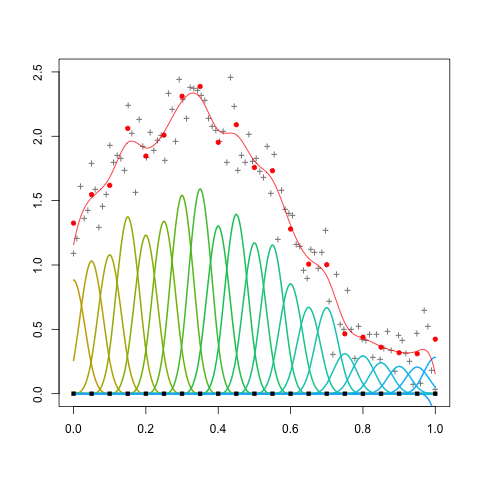
\includegraphics[scale=0.4]{pspline_pord2_xsmall_lambda.png}
  \label{fig:pspline_small_lambda}
\end{subfigure}
\begin{subfigure}{.5\textwidth}
  \centering
   \graphicspath{{img/}}
  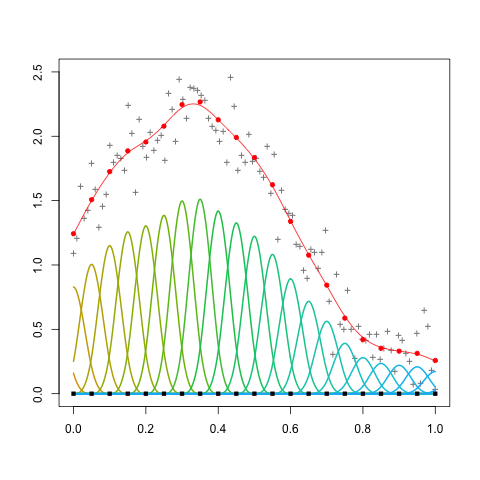
\includegraphics[scale=0.4]{pspline_pord2_small_lambda.png}
  \label{fig:pspline_small_lambda}
\end{subfigure}
\begin{subfigure}{.5\textwidth}
  \centering
   \graphicspath{{img/}}
  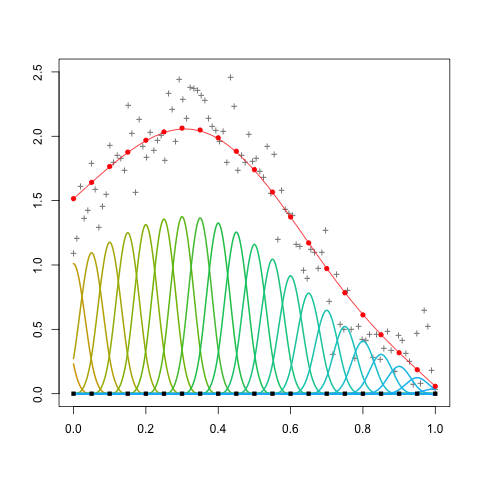
\includegraphics[scale=0.4]{pspline_pord2_medium_lambda.png}
  \label{fig:pspline_small_lambda}
\end{subfigure}
\begin{subfigure}{.5\textwidth}
  \centering
   \graphicspath{{img/}}
  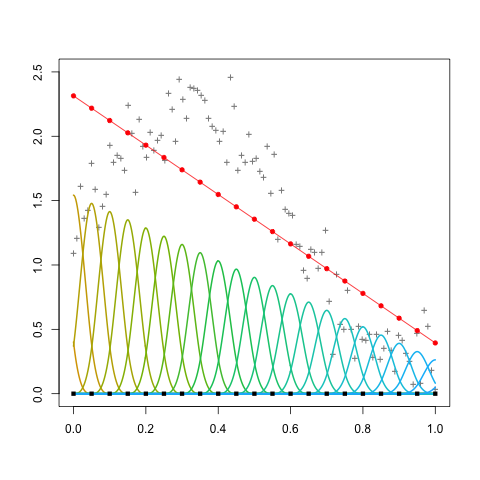
\includegraphics[scale=0.4]{pspline_pord2_large_lambda.png}
  \label{fig:pspline_small_lambda}
\end{subfigure}
\caption{\textit{Illustration of the impact of the second order difference penalty. The number of B-splines used is the same in each plot, with the value of the penalty parameter increasing from left to right and top to bottom across each plot. The red circles are the values of each of the B-spline coefficients; as the penalty increases, they form as smoother sequence as we move across the four plots, which results in a smoother fitted function. As the penalty parameter approaches infinity, the fit approaches a linear function as shown in the bottom right plot.}}
\label{fig:increasing-lambda-pspline-fits}
\end{figure}
The limiting P-spline fit approaches a polynomial as the smoothing parameter tends to infinity. Under a difference penalty of order $d$, the fitted function will approach a polynomial of degree $\left(d-1\right)$ for large values of the smoothing parameter as long as the degree of the B-splines is greater than or equal to $k$. Figure~\ref{fig:PS-difference-order-demo} demonstrates the impact of the order of the penalty on the fitted function as the smoothing parameter increases. To verify this mathematically, we need to use the relationship between the differenced coefficient sequence and the derivative of a B-spline. See Appendix~\ref{psplines-appendix}. Consider using the second-order difference penalty. When $\lambda$ is large, the penalty dominates the penalized likelihood, so that the minimizer $\theta$ must be such that $\sum\limits_{j}\left(\Delta^2\theta_j\right)^2$ is close to zero. Consequently, each of the individual second differences must also be nearly zero, and thus the second derivative of the fitted function must be close to zero over the entire domain.
\begin{figure}[H]
\begin{subfigure}{.5\textwidth}
  \centering
   \graphicspath{{img/}}
  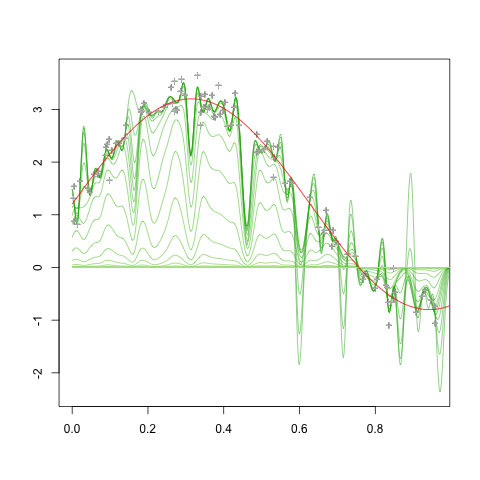
\includegraphics[scale=0.45]{PS_penalty_section_figure_6_order_0.png}
  %\label{fig:pspline_small_lambda}
\caption{$d=0$ }
\end{subfigure}
\begin{subfigure}{.5\textwidth}
  \centering
   \graphicspath{{img/}}
  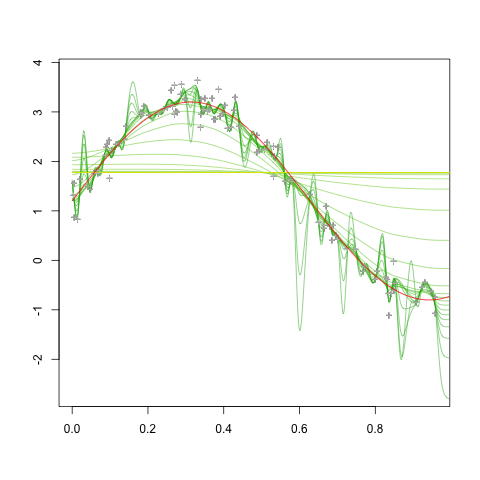
\includegraphics[scale=0.45]{PS_penalty_section_figure_6_order_1.png}
 % \label{fig:pspline_small_lambda}
\caption{$d=1$}
\end{subfigure}
\begin{subfigure}{.5\textwidth}
  \centering
   \graphicspath{{img/}}
  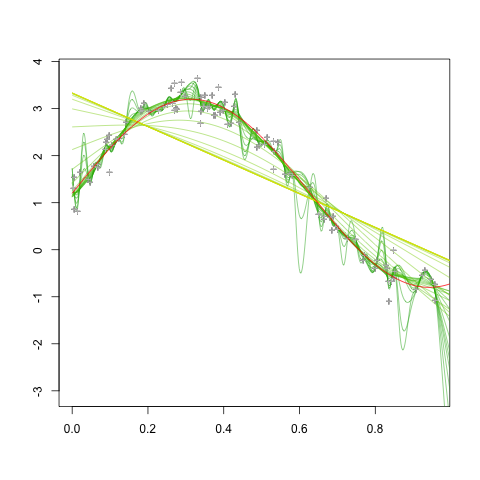
\includegraphics[scale=0.45]{PS_penalty_section_figure_6_order_2.png}
  %\label{fig:pspline_small_lambda}
\caption{$d=2$}
\end{subfigure}
\begin{subfigure}{.5\textwidth}
  \centering
   \graphicspath{{img/}}
  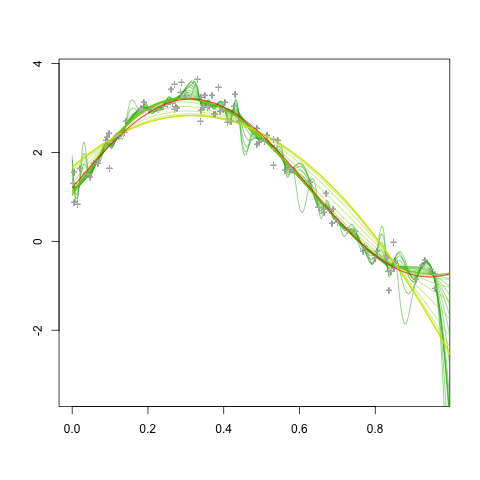
\includegraphics[scale=0.45]{PS_penalty_section_figure_6_order_3.png}
  %\label{fig:pspline_small_lambda}
\caption{$d=3$}
\end{subfigure}
\caption{\textit{Illustration of the impact of the order of the difference penalty. The number of B-splines used is the same in each plot, with the penalty parameter varying from across the same grid of values. The fitted curves in the upper left plot correspond to the difference penalty of order $0$, where $\vert D_0 \theta \vert^2 = \sum_{i} \theta_i^2$, analogous to ridge regression using the B-spline basis as regression covariates. The fitted curves approach polynomials of degree $d-1$ as $\lambda \rightarrow \infty$.}} \label{fig:PS-difference-order-demo}
\end{figure}


%%%%%%%%%%%%%%%%%%%%%%%%%%%%%%%%%%%%%%%%%%%%%%%%%%%%%%%%%%%%%%%%%%%%%%%%%%%%%%%%%%%%%%%%%%%
%%%%%%%%%%%%%%%%%%%%%%%%%%%%%%%%%%%%%%%%%%%%%%%%%%%%%%%%%%%%%%%%%%%%%%%%%%%%%%%%%%%%%%%%%%%
%%%%%%%%%%%%%%%%%%%%%%%%%%%%%%%%%%%%%%%%%%%%%%%%%%%%%%%%%%%%%%%%%%%%%%%%%%%%%%%%%%%%%%%%%%%
%%%%%%%%%%%%%%%%%%%%%%%%%%%%%%%%%%%%%%%%%%%%%%%%%%%%%%%%%%%%%%%%%%%%%%%%%%%%%%%%%%%%%%%%%%%
%%%%%%%%%%%%%%%%%%%%%%%%%%%%%%%%%%%%%%%%%%%%%%%%%%%%%%%%%%%%%%%%%%%%%%%%%%%%%%%%%%%%%%%%%%%
%%%%%%%%%%%%%%%%%%%%%%%%%%%%%%%%%%%%%%%%%%%%%%%%%%%%%%%%%%%%%%%%%%%%%%%%%%%%%%%%%%%%%%%%%%%
%%%%%%%%%%%%%%%%%%%%%%%%%%%%%%%%%%%%%%%%%%%%%%%%%%%%%%%%%%%%%%%%%%%%%%%%%%%%%%%%%%%%%%%%%%%
%%%%%%%%%%%%%%%%%%%%%%%%%%%%%%%%%%%%%%%%%%%%%%%%%%%%%%%%%%%%%%%%%%%%%%%%%%%%%%%%%%%%%%%%%%%

\section{The P-spline Estimator of the Generalized Autoregressive Varying Coefficient}

To extend the use of the difference penalty \eqref{eq:bspline-difference-penalty-1} to the bivariate setting, the only necessary modification to the one-dimensional differencing procedure is the addition of a second difference penalty so that there is a penalty for each variable, $l$ and $m$. Let $\Theta$ denote the $k_l \times k_m$ matrix of basis coefficients $\left\{\theta_{rc}\right\}$. For given $\Theta$, the fitted value $\phi\left(l,m\right)$ may be written 
\[
\sum_{r=1}^{k_l} \sum_{c=1}^{k_m} \theta_{rc} {B_l}_{_{r}}\left(l\right){B_m}_{_{c}}\left(m\right).
\]
\noindent
Let $\lambda = \left(\lambda_l, \lambda_m\right)$ denote the tuple of smoothing parameters for the $l$ and $m$ dimensions, respectively. We take $\phi_\lambda$ to be the minimizer of 
\begin{align} 
\begin{split}\label{eq:folded-difference-penalty-log-likelihood}
&-2\ell\left(\phi \vert Y_1,\dots, Y_N, \sigma^2\right) + J_{\lambda}\left(\phi\right) = \sum_{i=1}^N \sum_{j=2}^{p_i} \frac{1}{\sigma^{2}\left({t_{ij}}\right)} \left(y_{ij} - \sum_{k=1}^{j-1} \left( \sum_{r=1}^{k_l} \sum_{c=1}^{k_m} \theta_{rc} B_r\left(l_{ijk}\right)B_c\left(m_{ijk}\right)\right)y_{ik} \right)^2 \\ 
&\phantom{{} - 2\ell\left(\phi \vert Y_1,\dots, Y_N\right) + J_{\lambda}\left(\phi\right) =  } + \lambda_l \sum_{r=1}^{k_l} \vert\vert \theta_{r \cdot}  D_{d_{\ms l}} \vert\vert^2 + \lambda_m \sum_{c=1}^{k_m}\vert \vert  D_{d_{\ms m}} \theta_{\cdot c} \vert\vert^2,
\end{split}
\end{align}
\noindent
where $\theta_{r \cdot}$ and $\theta_{\cdot c}$ denote the $r^{th}$ row and $c^{th}$ column of $\Theta$, respectively. The second term in \eqref{eq:folded-difference-penalty-log-likelihood} imposes a difference penalty of order $d_{\ms l}$ on the rows of the coefficient matrix, while the third term places a difference penalty of order $d_{\ms m}$ on the columns. 

\bigskip

The penalized log likelihood is quadratic in $\theta = \left(\theta_{11}, \dots, \theta_{k_l, k_m} \right)'$. Demonstration of computation is simple if we express the coefficient matrix $\Theta$ in ``unfolded'' notation so that we can write the mean of the stacked response vector $Y$ as defined in \eqref{eq:stacked-response-vector} as in the usual multiple regression form
\begin{equation*}
E\left[Y \right] = X\mbox{vec}\left\{\phi\left( \bfv \right)\right\} = X B \theta,
\end{equation*}
\noindent
where $\theta = \mbox{vec}\left( \Theta \right)$ denotes the vectorized coefficient matrix constructed by stacking the columns of $\Theta$. The $\vert V \vert \times k_l k_m$ tensor product basis $B$ is constructed from the tensor product of the marginal B-spline bases defined in \citet{eilers2006fast} as the \textit{row-wise Kronecker product} of the individual bases:
\begin{equation} \label{eq:rowwise-kronecker-product}
B = B_m \square B_l = \left( B_m \otimes 1^\prime_{k_m} \right) \odot \left(1^\prime_{k_l} \otimes  B_l  \right).
\end{equation}
\noindent
The operator $\odot$ denotes the element-wise matrix product; $1_{k_l}$ ($1_{k_m}$) denotes the column vector of ones having length $k_l$ ($k_m$.) The operations in \eqref{eq:rowwise-kronecker-product} construct $B$ such that the $i^{th}$ row of $B_m\square B_l$ is the Kronecker product of the corresponding rows of $B_m$ and $B_l$. We can compactly express the penalty in \eqref{eq:folded-difference-penalty-log-likelihood} by writing
\begin{equation*} \label{eq:tensor-product-penalty}
\lambda_l \vert \vert P_l \theta \vert \vert^2 + \lambda_m \vert \vert P_m \theta \vert\vert^2
\end{equation*}
\noindent
where $P_l = I_{k_m} \otimes D'_{d_{\ms l}} D_{d_{\ms l}} $ and $P_m =  D'_{d_{\ms m}} D_{d_{\ms m}} \otimes I_{k_l}$. The $n_Y \times k_lk_m$  matrix $X$ is defined as before \eqref{eq:ar-design-matrix-1}. Then the log likelihood \eqref{eq:folded-difference-penalty-log-likelihood} can be written as
\begin{equation} \label{eq:tensor-pspline-objective-function}
-2\ell\left(\phi \vert Y_1,\dots, Y_N\right) + J_{\lambda}\left(\phi\right) = \left( Y - XB\theta\right)^\prime D^{-1}\left( Y - XB\theta\right)  + \lambda_l\vert\vert P_l \theta \vert\vert^2 + \lambda_m \vert\vert P_m \theta\vert \vert^2.
\end{equation}
\noindent
Taking derivatives and setting equal to zero gives normal equations:
\begin{equation} \label{eq:tensor-pspline-normal-equations}
\left[ \left(XB\right)^\prime D^{-1} XB +  \lambda_l P_l+ \lambda_m P_m\right]\theta = \left(X B\right)^\prime D^{-1}Y.
\end{equation}
\noindent
The solution $\phi_\lambda$ is given by $\phi_\lambda\left(\bfv\right) = \sum_{r=1}^{k_l} \sum_{c=1}^{k_m} \hat{\theta}_{rc} {B_l}_{_{r}}\left(l\right){B_m}_{_{c}}\left(m\right)$, where
\begin{equation} 
\hat{\theta} = \left[ \left(XB\right)^\prime D^{-1} XB +  \lambda_l P_l+ \lambda_m P_m\right]^{-1} \left(X B\right)^\prime D^{-1}Y.
\end{equation}
\noindent
We note that the size of the system of equations \eqref{eq:tensor-pspline-normal-equations} which determine the basis coefficients remains fixed at $k_l k_m$, even as the number of observations increases. The grid of regression coefficients can be recovered by arranging the elements of $\hat{\theta}$ into a matrix of $k_l$ columns having length $k_m$. The vector of fitted values is given by 
\begin{align}
\begin{split} \label{eq:pspline-smoothing-matrix}
\hat{Y} = AY  = X \left[ \left(XB\right)^\prime D^{-1} XB +  \lambda_l P_l+ \lambda_m P_m\right]^{-1} \left(X B\right)^\prime D^{-1}Y,
\end{split}
\end{align}
\noindent
where $A = X \left[ \left(XB\right)' D^{-1} XB +  \lambda_l P_l+ \lambda_m P_m\right] \left(X B\right)' D^{-1}$ is the ``smoothing'' matrix, analogous to the smoothing matrix $\tilde{A}$ \eqref{eq:smoothing-matrix-A-tilde} for the smoothing spline estimator in Chapter~\ref{SSANOVA-chapter}. Its use in smoothing parameter selection and model tuning is similar to the reproducing kernel Hilbert space framework, which we will discuss in the next section.

\bigskip

It is important to note that the construction of the tensor product basis $B$ and penalty matrix $P$ requires special care in this setting, where the domain of ${\phi}\left(l,m\right)$ is restricted to the region satisfying $0 \le s < t \le 1$, which is shown in Figure~\ref{fig:triangle-domain}.

\begin{figure}[H]
    \graphicspath{{img/}}
 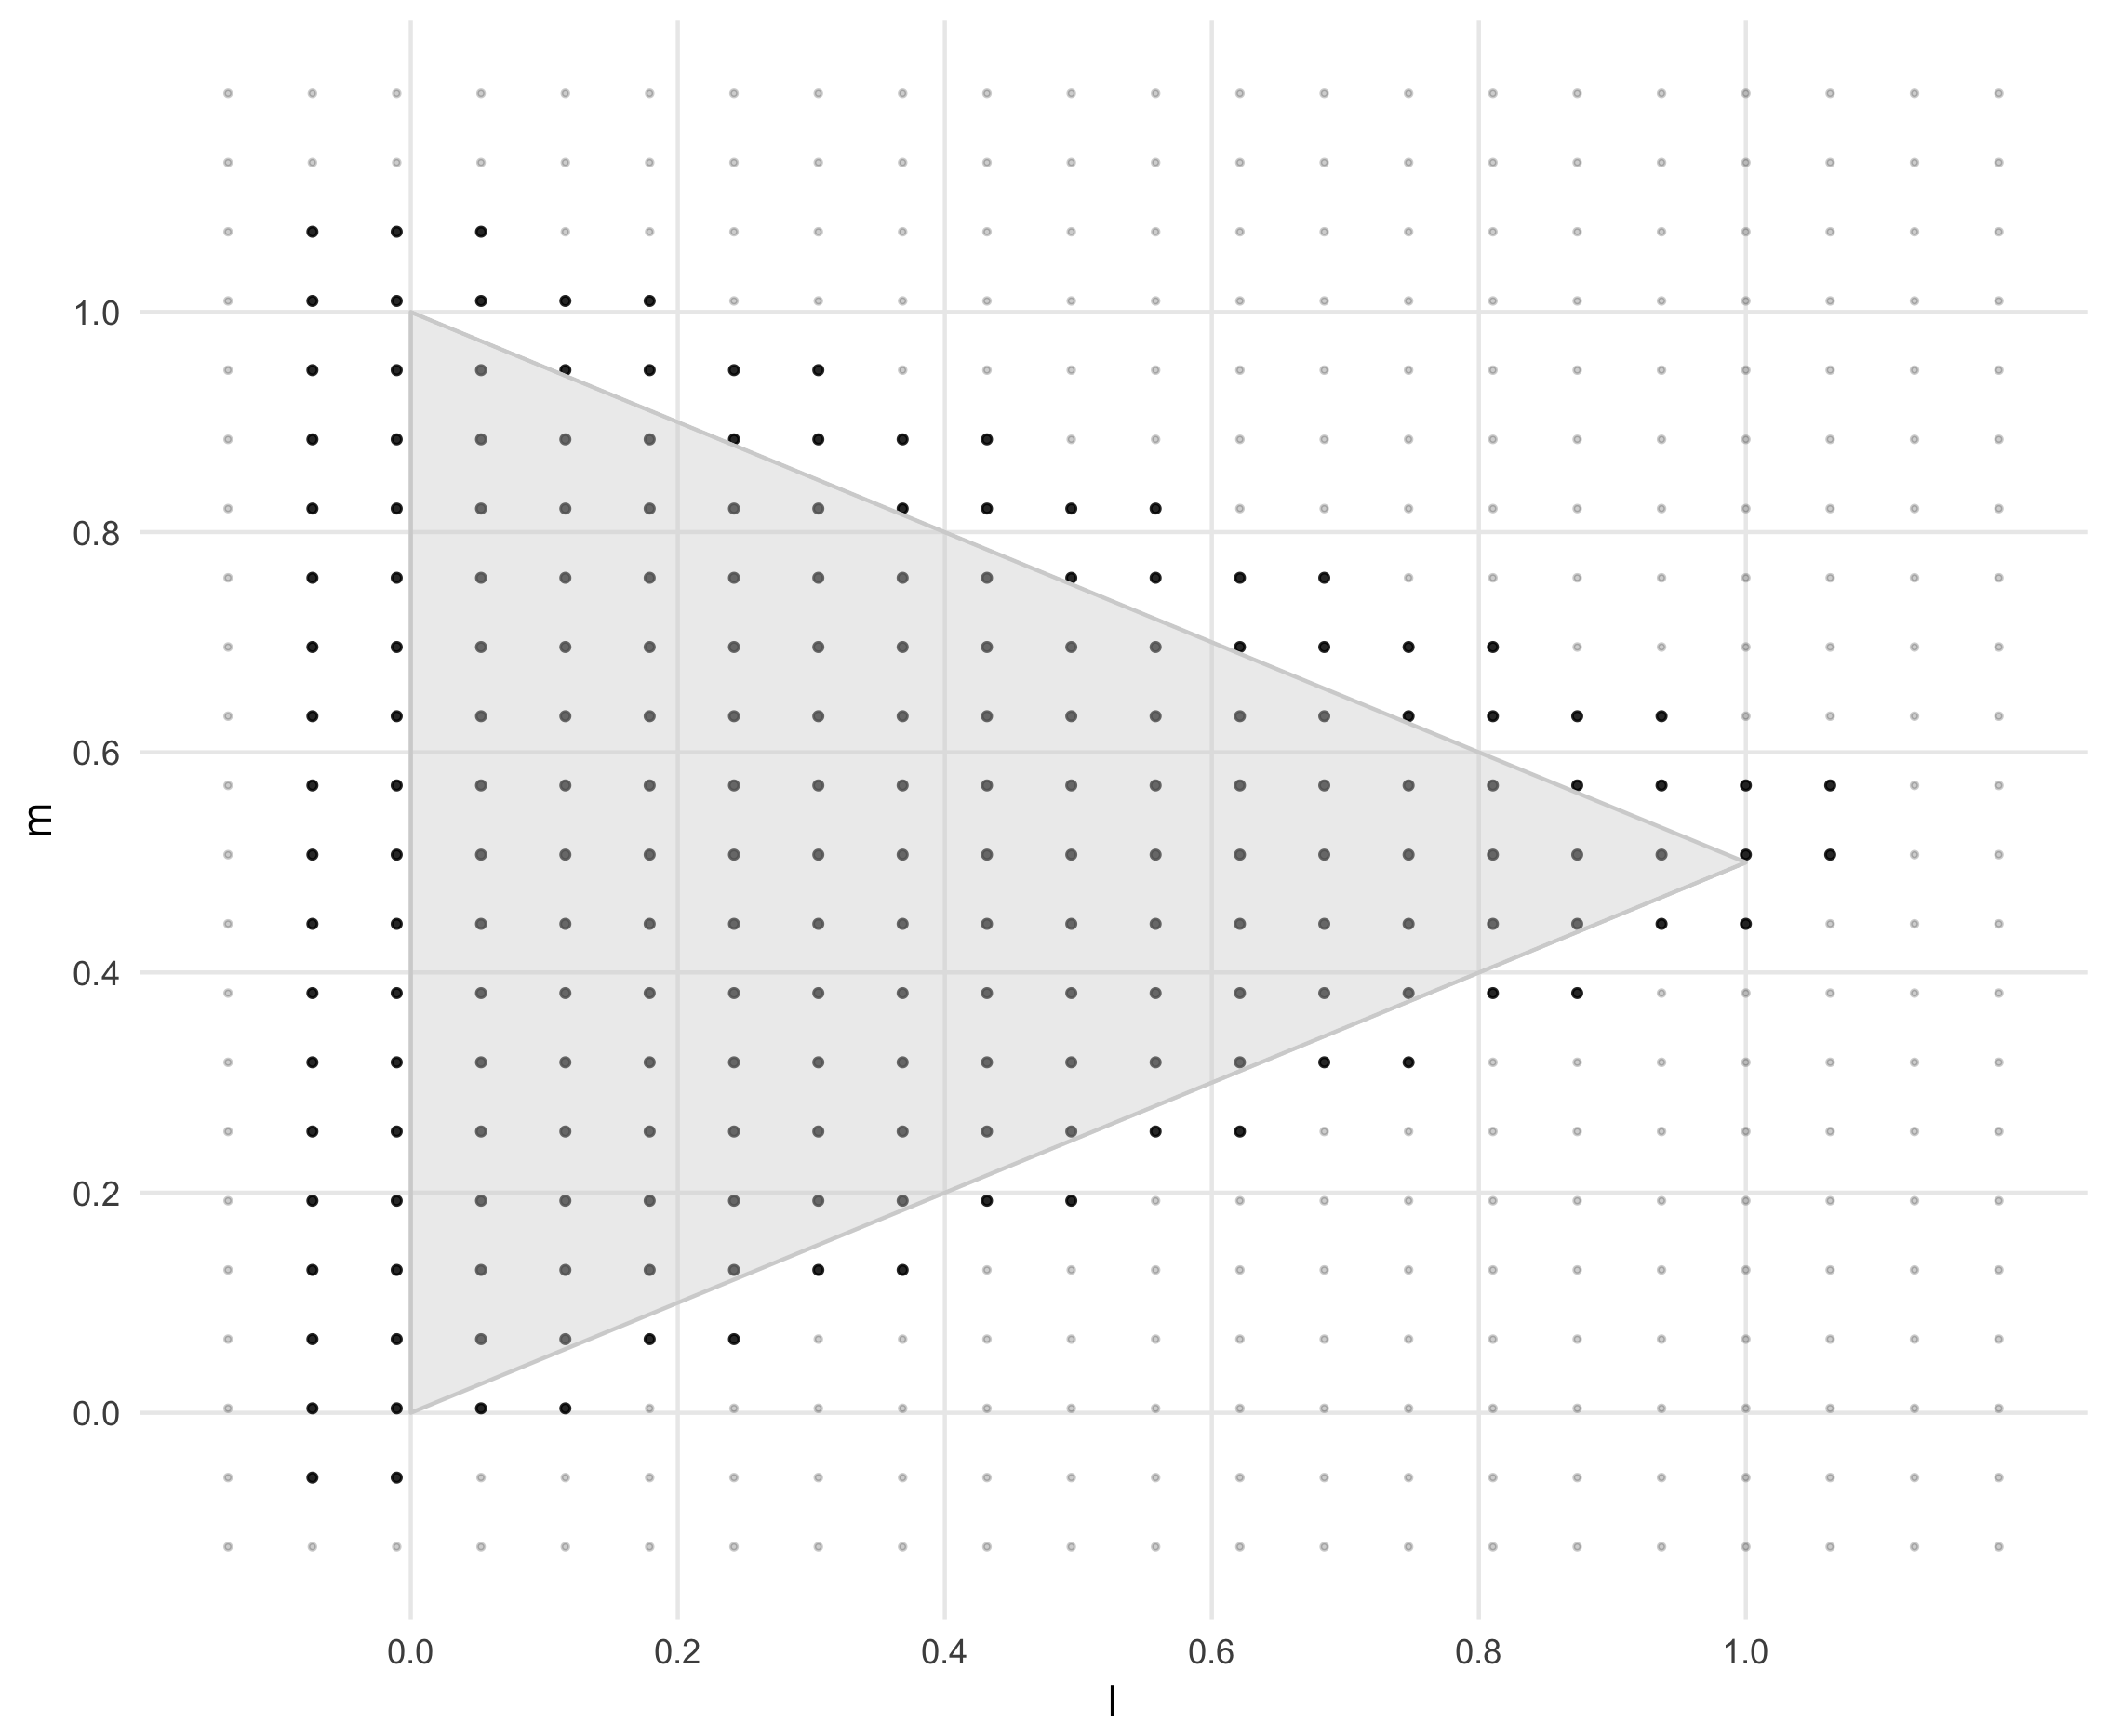
\includegraphics[scale=0.2]{knot-removal-on-triangle-domain.png}
 \caption{$\frac{l}{2} < m < 1 - \frac{l}{2}, \quad 0 < l < 1.$} \label{fig:triangle-domain}
 \end{figure}

When the tensor product basis is constructed on the regular grid defined by the cartesian product of the knots of the marginal bases $B_l$ and $B_m$, a large number of basis functions anchored are at knots near which we have no data, so there is little information about the corresponding basis coefficient. As a result, the resulting tensor product matrix can be ill-conditioned and solving \eqref{eq:tensor-pspline-normal-equations} results in singularities. In this case, the quality of the estimator can suffer terribly. To correct for this instability, one can simply remove the knots corresponding to tensor products functions which do not overlap with the function domain from the basis, $B$, and trimming the penalty matrices $P_l$ and $P_m$ as needed. With the trimmed basis and penalties, optimization can be carried out as previously discussed. 

\bigskip

Triangular B-splines are a new tool for modeling complex objects with nonrectangular topology. The scheme is based on blending functions and control points, and lets us model piecewise pol
Bivariate B-splines are useful for smoothing over arbitrary domains, making them a natural alternative for the construction of a basis for $\bfv = \left(l,m\right)$. Multidimensional B-splines are well-developed by mathematicians, but they are rarely used in the statistical community. To smooth over non-rectangular domains, the domain is approximated by a set of triangles, or a triangulation, where each triangle is defined by its three vertices. The B-splines are defined according to a set of triples which correspond to set of knots over the bivariate domain. See \citet{dahmen1992blossoming} and \citet{seidel1991symmetric} for details. 

%%%%%%%%%%%%%%%%%%%%%%%%%%%%%%%%%%%%%%%%%%%%%%%%%%%%%%%%%%%%%%%%%%%%%%%%%%%%%%%%%%%%%%%%%%%
%%%%%%%%%%%%%%%%%%%%%%%%%%%%%%%%%%%%%%%%%%%%%%%%%%%%%%%%%%%%%%%%%%%%%%%%%%%%%%%%%%%%%%%%%%%
%%%%%%%%%%%%%%%%%%%%%%%%%%%%%%%%%%%%%%%%%%%%%%%%%%%%%%%%%%%%%%%%%%%%%%%%%%%%%%%%%%%%%%%%%%%
%%%%%%%%%%%%%%%%%%%%%%%%%%%%%%%%%%%%%%%%%%%%%%%%%%%%%%%%%%%%%%%%%%%%%%%%%%%%%%%%%%%%%%%%%%%
%%%%%%%%%%%%%%%%%%%%%%%%%%%%%%%%%%%%%%%%%%%%%%%%%%%%%%%%%%%%%%%%%%%%%%%%%%%%%%%%%%%%%%%%%%%
%%%%%%%%%%%%%%%%%%%%%%%%%%%%%%%%%%%%%%%%%%%%%%%%%%%%%%%%%%%%%%%%%%%%%%%%%%%%%%%%%%%%%%%%%%%
%%%%%%%%%%%%%%%%%%%%%%%%%%%%%%%%%%%%%%%%%%%%%%%%%%%%%%%%%%%%%%%%%%%%%%%%%%%%%%%%%%%%%%%%%%%
%%%%%%%%%%%%%%%%%%%%%%%%%%%%%%%%%%%%%%%%%%%%%%%%%%%%%%%%%%%%%%%%%%%%%%%%%%%%%%%%%%%%%%%%%%%


%%==============================================================================================================================================
%%==============================================================================================================================================
%%==============================================================================================================================================
%%==============================================================================================================================================
%%==============================================================================================================================================
%%%==============================================================================================================================================


%%==============================================================================================================================================
%%==============================================================================================================================================
%%==============================================================================================================================================
%%==============================================================================================================================================
%%==============================================================================================================================================
%%==============================================================================================================================================

%%==============================================================================================================================================
%%==============================================================================================================================================
%%==============================================================================================================================================
%%==============================================================================================================================================
%%==============================================================================================================================================
%%==============================================================================================================================================

%\subsection{The reguarlized MLE for $\phi$ via tensor product P-splines}
%% \subfile{chapter-3-subfiles/chapter-3-tensor-product-pspline-MLE}
%To extend the P-spline framework to allow estimation of a bivariate function, $\phi$, we simply need to equip the $l$ and $m$ axes each with a B-spline basis. A basis for the varying coefficient function is constructed taking the tensor product of the two marginal bases. Let 
%\[
%B_{1}\left(l\right),\dots, B_{K}\left(l\right)  \mbox{ and } B_{1}\left(m\right),\dots, B_{L}\left(m\right)
%\]
%denote the B-spline bases for $l$ and $m$, each having a set of equally spaced knots along their respective domain. It is worth noting that while we have chosen not to distinguish between $\left\{ B_k \right\}$ and $\left\{ {B}_l \right\}$ for the sake of brevity, one is free to specify a different basis for each dimension either by using different order B-spline or, of course, using different numbers of knots, and hence entirely different knot sequences since P-splines rely on bases with equally spaced knots. The tensor product basis functions
%\begin{equation*}
%T_{jk}\left(l,m\right) = B_j\left(l\right){B}_k\left(m\right)
%\end{equation*}
%\noindent
%carve the $l$-$m$ domain into rectangles.  Figure~\ref{fig:sparse_bicubic_BS_basis} shows a thinned tensor product basis $\left\{ T_{kl} \right\}$; a portion of the basis was omitted to eliminate overlapping of the basis functions so that the reader can identify individual tensor products. Each ``hill'' in Figure~\ref{fig:sparse_bicubic_BS_basis} is associated with an unknown coefficient $\theta_{ij}$ which determines the height of the hill. For a given knot grid, we can approximate a surface by
%
%\begin{equation} \label{eq:varying-coefficient-tensor-product-expansion}
%\phi\left(l,m\right) = \sum_{i=1}^K \sum_{j=1}^L \theta_{ij} B_{i}\left(l\right) B_{j}\left(m\right), 
%\end{equation}
%\noindent
%and the function evaluated at the observed $\left(l_{ijk}, m_{ijk}\right)$ may be written 
%\begin{equation*} 
%\vphistar = B_m \Theta B_l^\prime
%\end{equation*}
%\noindent 
%where $\Theta$ denotes the $K \times L$ matrix of tensor product coefficients, with elements $\theta_{ij}$.
%
%\begin{figure}[H]
%\centering
% \graphicspath{{img/}}
%  \includegraphics[width=4in, height=4in]{bicubic_basis_function.png}
% 
%% 
% \subsection{Regularization with difference penalties} \label{subsection:univariate-psplines}
%
%The minimizer of \eqref{eq:loglikelihood} honors the fidelity to the data, so to balance the complexity of the fitted function with the goodness of fit to the data, we can append a penalty to the negative log likelihood to control the fitted function. By using rich B-spline bases for $l$ and $m$ alongside discrete difference penalties on the spline coefficients, we can achieve as much smoothness of the fitted function in both the $l$ and $m$ dimensions as desired. \cite{o1986statistical} was the first to propose using a rich B-spline basis and using a penalty to restrict the flexibility of the fitted curve, like \cite{wahba1990spline} applying a penalty to the second derivative of the fitted curve:
%\[
%J = \int_0^1 \left[ f^{\prime \prime}\left(l\right)\right]^2\;dx.
%\]
%
%For a B-spline of the form
%\[
%f\left(x\right) = \sum\limits_{j=1}^n \theta_i B_j\left(x\right),
%\]
%one can derive a banded matrix $P$ using the properties of B-splines such that 
% \[
% J = \theta^\prime P \theta
% \] 
% \noindent
% where $\theta = \left(\theta_1,\dots, \theta_n\right)$. The $i$-$j^{th}$ element of $P$ is given by
% \[
% p_{ij} = \int_0^1 B_i^{\prime \prime} \left( x \right)B_j^{\prime \prime} \left( x \right)\;dx.
% \]

%As discussed in Section 2, we can define an entire class of functional autoregressive models using only the $l$ direction, and additionally, as discussed in Section 3, there is a natural expectation about the functional form of the autoregressive coefficient function (and hence covariance) as a function of $l$. The use of smoothing splines to estimate $\phi$ outlined in Section~\ref{} yields smooth null models, but smoothness of the elements of the Cholesky factor alone may not lead to desirable structure in the inverse covariance matrix.  

%
%These approaches implicitly adopt different notions of sparsity. Like \cite{huang2006covariance} and \cite{levina2008sparse}, our aim is to regularize the inverse of the covariance matrix through the Cholesky factor. Expressing the varying coefficient function using a tensor product basis expansion builds the foundation for a flexible estimation framework within which employing multiple notions of smoothness is simple and straightforward. 
%
%
%In some applications, it is useful to work with third and fourth order differences, since for large values of $\lambda$, the fitted curve approaches a parametric polynomial model. This may be of particular interest in the context of estimating the elements of the Cholesky factor, as many have proposed simple parametric functions of lag only for $\phi$, such as low order polynomials. See \cite{pourahmadi1999joint}. However, with the use of higher order derivatives, the computation of $P$ is nontrivial and becomes very tedious. \cite{eilers1996flexible} were the first to propose P-splines, or \emph{penalized B-splines}, as an approach to nonparametric regression. P-splines circumvent complexity associated with constructing such penalty matrices by omitting derivatives and integrals altogether, replacing them with finite differences and sums. 
%
%Instead, flexibility of the fitted function is controlled by using a discrete penalty matrix based on finite difference formulas. Smoothness of the fitted function is achieved by first using a rich B-spline basis with equally spaced knots to purposefully overfit the smooth coefficient vectors; this eliminates the difficulty of choosing the optimal set of knots. Then by attaching a difference penalty to the goodness of fit measure, one may prevent overfitting and make a potentially ill-conditioned fitting procedure a well-conditioned one. The finite difference penalty is simple to compute and can be handled mechanically for any order of the differences. Since it is easily introduced into regression equations, it is feasible to evaluate the impact of different orders of the differences on the fitted model.  Using the properties of B-splines, it is straightforward to show that the difference penalty of order $d$ is a good discrete approximation to the integrated square of the $d^{th}$ derivative, so little is lost by replacing the derivative-based penalty with
%
%\begin{equation} \label{eq:bspline-difference-penalty}
%J_d\left( f \right) = \sum_{j=d}^n \left(\Delta^d \theta_j\right)^2
%\end{equation} 
%\noindent
%where $\theta = \left( \theta_1,\dots,\theta_n \right)$. Let $D_d$ denote the matrix difference operator: $D_d\theta = \Delta^d \theta$, where
%
% \begin{align*}
% \Delta \theta_j &= \theta_j - \theta_{j-1}, \quad  \Delta^2 \theta_j = \Delta\left(\Delta \theta_j\right) = \theta_j - 2\theta_{j-1} + \theta_{j-2}
% \end{align*}
%\noindent 
%In general,
%\begin{equation*}
%\Delta^d \theta_j = \Delta\left(\Delta^{d-1} \theta_j \right).
%\end{equation*} 
%\noindent
%Then, \eqref{eq:bspline-difference-penalty} can be written in terms of the squared norm of the difference operator applied to the vector of B-spline coefficients:
%\begin{align} 
%\begin{split} \label{eq:bspline-difference-penalty-vector-form}
%J_d\left( f \right) &= \vert \vert D_d\theta \vert \vert^2 \\
%&= \theta^\prime P_d \theta
%\end{split}
%\end{align}
%\noindent
%where $P_d = D_d^\prime D_d$.  To examine the connection between the second-derivative penalty to the penalty on second-order differences of the B-spline coefficients, we only need to employ straightforward calculus and exploit the recursive property of the B-spline basis functions:
%
%\begin{equation*} 
%\int_0^1 \left[ f^{\prime \prime}\left(x\right)\right]^2\;dx = \int_{0}^{1} \left\{ \sum\limits_{j=1}^n  \theta_j B_{j3}^{\prime \prime} \left(l\right) \right\}^2\; dl.
%\end{equation*}
%\noindent
%The derivative properties of B-splines permits this to be written as 
%\begin{equation*} \label{eq:second-derivative-bspline-penalty}
%\int_0^1 \left[ f^{\prime \prime}\left(x\right)\right]^2\;dx =  \int_{0}^{1}  \bigg[ \sum\limits_{j=1}^n \sum\limits_{k=1}^n \Delta^2 \theta_j \Delta^2 \theta_k B_{j1}\left(l\right)B_{k,1}\left(l\right)\bigg]\; dl  . 
%\end{equation*}
%\noindent
%Most of the cross products of $B_{j1}\left(x\right)$ and $B_{k,1}\left( x \right)$ vanish since B-splines of degree 1 only overlap when $j$ is $k-1$, $k$, or $k+1$. Thus, we have that
%\begin{align}
%\begin{split}
%\int_0^1 \left[ f^{\prime \prime}\left(x\right)\right]^2\;dx  = {} &  \int_0^1 \bigg[ \left\{ \sum\limits_{j=1}^n   \Delta^2 \theta_j  B_j\left(l,1\right)  \right\}^2  + 2 \sum_{j}\Delta^2 \theta_j\Delta^2 \theta_{j-1}B_j\left(l,1\right)B_{j-1}\left(l,1\right) \bigg]\; dl \\ 
%= {} & \sum \limits_{j=1}^n  \left( \Delta^2\theta_j \right)^2 \int_0^1 B_j^2\left(l,1\right)\;dl \\
%   &{} \;\;\;\;\;\;\;\;\;\;\;\;\;\;\;\;\;\; + 2 \sum\limits_{j=1}^n \Delta^2 \theta_j\Delta^2 \theta_{j-1} \int_0^1 B_j\left(l,1\right)B_{j-1}\left(l,1\right)\;dl 
%\end{split}
%\end{align}
%\noindent
%which can be written as
%\begin{equation} \label{eq:derivative-penalty-difference-penalty-connection}
%\int_0^1 \left[ f^{\prime \prime}\left(x\right)\right]^2\;dx  = c_1 \sum\limits_{j=2}^n \left( \Delta^2 \theta_j\right)^2 + c_2 \sum\limits_{j=3}^n \Delta^2 \theta_j\Delta^2 \theta_{j-1}
%\end{equation}
%\noindent
%Given a set of equidistant knots, the constants $c_1$ and $c_2$ are given by
%\begin{equation}
%\begin{split}
%c_1 & =   \int_0^1 B_{j1}^2\left(x\right) dx\\
%c_2 & = \int_0^1 B_{j1}\left(x\right)B_{j-1,1}\left(x\right) dx.
%\end{split}
%\end{equation}
%
%This gives us that the traditional smoothness penalty on the squared second derivative can be written as a linear combination of a penalty on the second-order differences of the B-spline coefficients \eqref{eq:bspline-difference-penalty} and the sum of the cross products of neighboring second differences. The second term in \eqref{eq:derivative-penalty-difference-penalty-connection} leads to a complex objective function when minimizing the penalized likelihood, where seven adjacent spline coefficients occur, as opposed to five if only the first term in \eqref{eq:derivative-penalty-difference-penalty-connection} is used in the penalty. The added complexity is a consequence of overlapping B-splines, which quickly increases when using higher order differences and higher order B-splines. We can seamlessly augment the likelihood with the difference penalty to achieve smooth fitted functions without the complexity posed by the derivative-based penalty.
%%citet{chen2011efficient}, citet{pourahmadi1999joint}, and citet{pourahmadi2002dynamic} have elicited parametric models for the generalized autoregressive coefficients, letting the GARPs depend only on the distance between two time points.
%
%A smoother sequence of coefficients leads to a smoother curve, as illustrated in Figure~\ref{fig:second_ord_PS_pen_SML_lambda}.  The relationship between P-spline curves and their coefficients is easily characterized if we consider the coefficients as the skeleton of the function, and draping the B-splines over them puts the flesh on the bones. As long as the coefficient sequence is smooth, the number of basis functions (and coefficients) is unimportant since the penalty ensures the smoothness of the skeleton and that the fitting procedure is well-conditioned. Figure~\ref{fig:overcomplete_basis_pspline} illustrates this utility of the penalty for simulated data; there are $m=10$ observations and $60$ cubic B-splines. This property of P-splines cannot be overly appreciated because it frees us from the concern of choosing the optimal set of knots. Unless computational constraints are of concern, which is possible with large models, it is prudent to use even more B-splines. Figure~\ref{fig:PS_penalty_section_figure_2} shows how the fitted function changes as the tuning parameter varies when the data are sparsely sampled. P-splines enjoy a number of additional advantageous properties, many of which are inherited from the attractive properties of B-splines. See \cite{eilers1996flexible}  for a detailed presentation. 
%
%\begin{figure}[H] \label{fig:PS-smoothing-figure-1}
%\begin{subfigure}{.5\textwidth}
%  \centering
%   \graphicspath{{img/}}
%  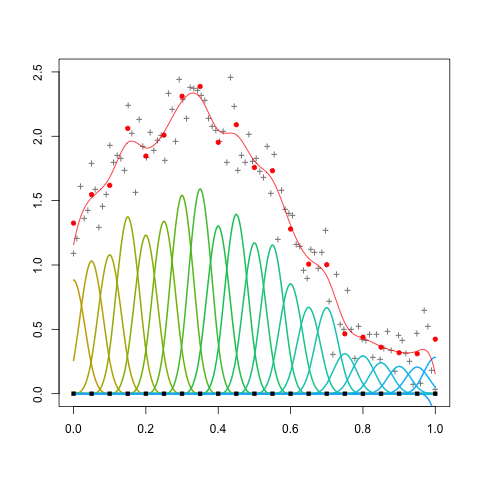
\includegraphics[scale=0.5]{pspline_pord2_xsmall_lambda.png}
%  \label{fig:pspline_small_lambda}
%\end{subfigure}
%\begin{subfigure}{.5\textwidth}
%  \centering
%   \graphicspath{{img/}}
%  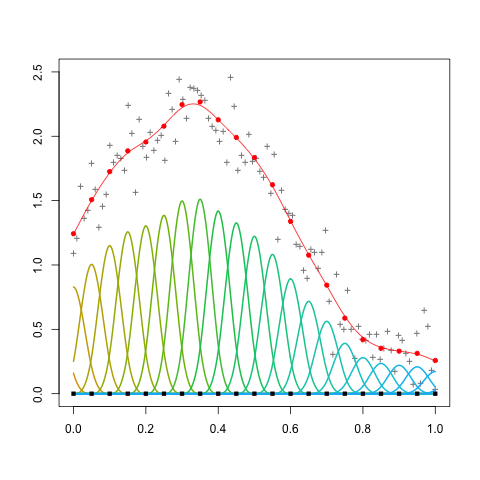
\includegraphics[scale=0.5]{pspline_pord2_small_lambda.png}
%  \label{fig:pspline_small_lambda}
%\end{subfigure}
%\begin{subfigure}{.5\textwidth}
%  \centering
%   \graphicspath{{img/}}
%  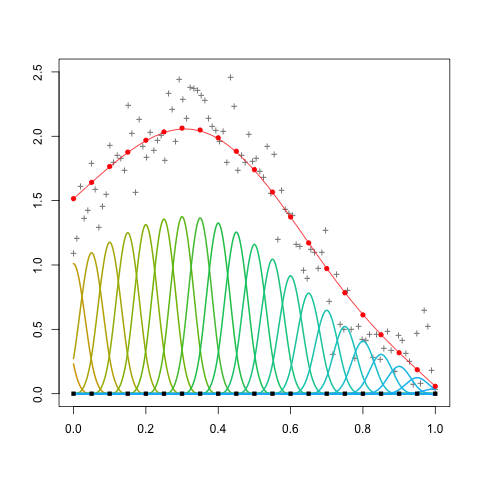
\includegraphics[scale=0.5]{pspline_pord2_medium_lambda.png}
%  \label{fig:pspline_small_lambda}
%\end{subfigure}
%\begin{subfigure}{.5\textwidth}
%  \centering
%   \graphicspath{{img/}}
%  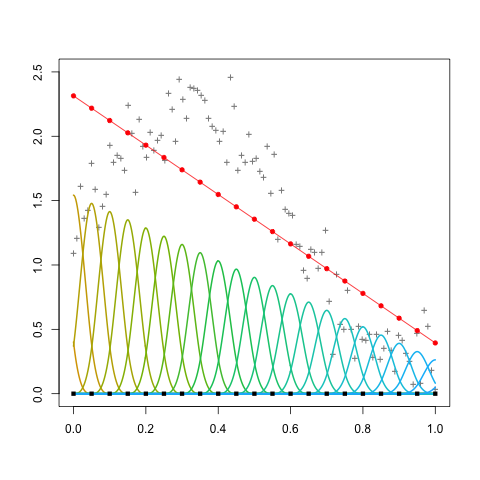
\includegraphics[scale=0.5]{pspline_pord2_large_lambda.png}
%  \label{fig:pspline_small_lambda}
%\end{subfigure}
%\caption{\textit{Illustration of the impact of the second order difference penalty. The number of B-splines used is the same in each plot, with the value of the penalty parameter increasing from left to right and top to bottom across each plot. The fitted curve in the upper left plot is the most ``wiggly'' of any of the fits, as the penalty plays the weakest roll in the fitted coefficients there. The red circles are the values of each of the B-spline coefficients; as the penalty increases, they form as smoother sequence as we move across the four plots, which results in a smoother fitted function. As the penalty parameter approaches infinity, the fit approaches a linear function as shown in the bottom right plot.}}
%\label{fig:second-ord-PS-pen-SML-lambda}
%\end{figure}
%%==============================================================================================================================================
%%==============================================================================================================================================
%%==============================================================================================================================================
%%==============================================================================================================================================
%%==============================================================================================================================================
%%==============================================================================================================================================

% \begin{columns}
%\begin{column}{0.5\textwidth}
%Equip $l$ and $m$ with
%\begin{align*}
%B_{1}\left(l\right),\dots, B_{K}\left(l\right),\\
%B_{1}\left(m\right),\dots, B_{L}\left(m\right)
%\end{align*}
%to build
%\begin{equation*}
%T_{jk}\left(l,m\right) = B_j\left(l\right){B}_k\left(m\right)
%\end{equation*}
%  \end{column}
%\begin{column}{0.5\textwidth}  %%<--- here
%    \begin{center}
%    \begin{figure}
%    \graphicspath{{img/}}
% 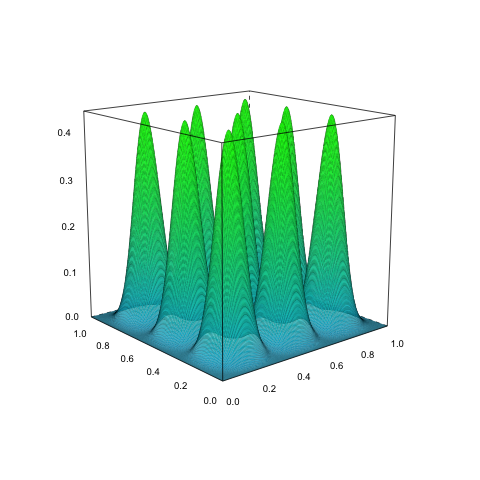
\includegraphics[width=4cm]{sparse_bicubic_basis}
% \caption{A ``thinned'' tensor product basis}
% \end{figure}
%     \end{center}
%\end{column}
%\end{columns}
%\vspace{0.3cm}
%\begin{equation*}
%\phi\left(l,m\right) = \sum_{i=1}^K \sum_{j=1}^L \theta_{ij} B_{i}\left(l\right) B_{j}\left(m\right)
%\end{equation*}
%
 
%The parameters of the functional autoregressive model given by \eqref{eq:MyModel} define the elements of the precision matrix $\Omega$, rather than the elements of $\Sigma$ itself. It is well known that if we let $Y = \left(Y_1, \dots, Y_m\right)^\prime$ denote the random vector having joint distribution with mean zero and covariance matrix $\Sigma$, then the elements of $\Sigma^{-1}=\Omega$, $\left\{ \omega_{ij} \right\}$ may be interpreted as partial covariances between the elements of $Y$. This suggests shrinking $\phi$ to zero for large values of $l$. One can show that if $T$ has $k$ non-zero diagonals, then the middle $k$ diagonals of $\Sigma^{-1}$ are non-zero.  

%For ease of exposition, we first focus our attention on the estimation of $\phi$ assume that $\sigma^2\left(t\right)$ is fixed and known. Estimation of the innovation variance function is presented in Section~\ref{section:variance-estimation}. In the case that subjects share a common set of observation times $t_1 < \dots < t_m$,  it is well known that the MLE for $\Sigma$, $S = \sum_{i=1}^N y_i y_i^\prime$ is highly unstable in high dimensions, a condition that is potentially worsened when one or more subjects has at least one observation time that is unique from the set of observation times common across subjects. To mitigate instability due to high dimensionality and simultaneously permit the estimation of $\phi\left(\cdot,\cdot\right)$ as a smooth bivariate function, we obtain a covariance estimator by applying bivariate smoothing of the elements of the Cholesky factor. 

%%====================================================================================

\section{Smoothing Parameter Selection}

%\subfile{chapter-3-subfiles/chapter-3-tensor-product-pspline-model-selection}
As with the RKHS framework and accompanying smoothing spline representation, the smoothing matrix  
\begin{equation*}\label{eq:pspline-smoothing-matrix}
A_\lambda = X \big( \left(X B\right)' D^{-1} XB +  \lambda_l P_l+ \lambda_m P_m \big)^{-1}\left(X B\right)' D^{-1}
\end{equation*}
\noindent
and its properties play an integral role in selecting the optimal smoothing parameter in any regularized regression, including the P-spline framework. We discussed the leave-one-subject-out cross validation score \eqref{eq:LOSOCV} and its computationally efficient approximation \eqref{eq:approx-losocv} in Chapter~\ref{SSANOVA-chapter}, which rely directly on the smoothing matrix for calculation. The model selection criteria discussed in Section~\ref{gaussian-unbiased-risk-estimate}  can be calculated as in the smoothing spline setting by replacing $\tildeA_{\lambda,\bftheta}$ with $A_\lambda$. For detailed discussion of P-spline model selection with respect to multiple smoothing parameters, see \cite{wood2017generalized}.

\bigskip

%Summarizing the complexity of a fitted P-spline is non-trivial; it requires the simultaneous consideration of the smoothing parameters, the number of basis functions in the B-spline basis, and the order of the difference penalties. To assess model complexity, \cite{eilers1996flexible} follow \cite{hastie1990generalized}, who use the trace of the smoothing matrix as an approximation of the \textit{effective dimension} (ED) of a linear smoother. The effective (model) dimension is defined as 
%
%%\begin{align}
%\begin{equation} \label{eq:trace-of-the-smoothing-matrix}
%\textup{ED} = \textup{tr}\left( A_\lambda \right) = \textup{tr}\bigg( X\left( \left(XB\right)^\prime D^{-1}XB +  \lambda_l P_l+ \lambda_m P_m\right)^{-1} \left(X B\right)^\prime D^{-1}  \bigg)
%\end{equation}
%%\end{align}
%
%\noindent
%The ED combines the effect of the smoothing parameter, the number of basis functions, and the differencing order, and it is easy to compute. When the number of basis functions is significantly smaller than the sample size, it is advantageous to use the cyclic property of the trace: 
%
%\begin{align*}
%\textup{tr}\left( A_\lambda \right) &= \textup{tr}\bigg( X\left( \left(XB\right)^\prime D^{-1}XB +  \lambda_l P_l+ \lambda_m P_m\right)^{-1} \left(X B\right)^\prime D^{-1}  \bigg)\\
%&= \textup{tr}\bigg( \left(X B\right)^\prime D^{-1}  X\left( \left(XB\right)^\prime D^{-1}XB +  \lambda_l P_l+ \lambda_m P_m\right)^{-1} \bigg),
%\end{align*}
%
%\noindent
%which requires computing the trace of a $k_lk_m \times k_lk_m$ matrix, which is computationally more economical when the total number of basis functions is smaller than the total number of observations. This approach to approximating the effective model dimension is also consistent with \cite{ye1998measuring}, who constructed a generalization of the concept of a model's degrees of freedom using the idea that the degrees of freedom can also be interpreted as the sum of the sensitivity of each fitted value with respect to the corresponding observed value.
%
%\bigskip
%
%Using the eigenstructure of the smoothing matrix, one can show that as the smoothing parameters tend to infinity, the effective dimension approaches $d_l + d_m$, the sum of the order of the differencing operators for $l$ and $m$. Let
%
%\begin{equation*}
%Q = \left(X B\right)^\prime D^{-1} XB \qquad \mbox{and} \qquad Q_\lambda = \lambda_l P_l + \lambda_m P_m.
%\end{equation*}
%
%Again using cyclic property of the trace, we can write
%\begin{align*}
%%\begin{split}
%\mbox{tr}\left(A_\lambda \right) &= \mbox{tr}\bigg[ \left(Q + Q_\lambda \right)^{-1}Q \bigg]\\
%&=\mbox{tr}\bigg[ Q^{1/2}\left(Q + Q_\lambda \right)^{-1}Q^{1/2} \bigg] \\
%&=\mbox{tr}\bigg[\left(I + Q^{-{1/2}}Q_\lambda Q^{-{1/2}} \right)^{-1} \bigg]
%%\end{split}
%\end{align*}
%
%\noindent
%Finally we have that
%\begin{equation*}
%\mbox{tr}\left(A_\lambda \right) = \mbox{tr}\bigg[\left(I + \lambda Q^{-{1/2}}Q_\lambda Q^{-{1/2}}  \right)^{-1} \bigg] = \sum_{j=1}^{k_lk_m} \frac{1}{1 + \lambda \gamma_j},
%\end{equation*}
%
%\noindent
%where $\gamma_j$, $j=1,\dots,k_lk_m$ are the eigenvalues of $Q^{-{1/2}}Q_\lambda Q^{-{1/2}}$. The matrix constructed from the sum of the penalty terms, $Q_\lambda$, has exactly $d_l + d_m$ eigenvalues equal to zero. Hence, $Q^{-{1/2}}Q_\lambda Q^{-{1/2}} $ has $d_l + d_m$ eigenvalues equal to zero, so for large $\lambda$, only the $d_l + d_m$ terms with $\gamma_j=0$ contribute to the sum which gives the trace of $A_\lambda$. Then
% 
% \[
%\lim_{\lambda \rightarrow \infty  } \mbox{tr}\left(A_\lambda\right) = d_l + d_m.
% \]
%
%%A further simplification of \eqref{eq:hat-matrix-trace}
%%
%%\begin{align*} 
%%\left(B^T B + \lambda D^T D \right)^{-1} B^T B &= \left(B^T B + \lambda D^T D \right)^{-1} \left( B^T B + \lambda D^T D - \lambda D^T D\right) \nonumber \\
%%&= I - \lambda\left(B^T B + \lambda D^T D \right)^{-1} D^T D \label{eq:cyclic_hat_matrix_simplification}
%%\end{align*}
%%
%%\begin{align*} 
%%\left[\left(WB\right)^\prime D^{-1}WB +  \lambda_l P_l+ \lambda_m P_m\right]^{-1} \left(W B \right)^\prime D^{-1} WB  &= \left[\left(WB\right)^\prime D^{-1}WB +  \lambda_l P_l+ \lambda_m P_m\right]^{-1}\left(W B \right)^\prime D^{-1} \times \\
%%&\mbox{\;\;\;\;\;\;\;\;\;\;\;\;\;\;\;\;\;\;\;\;\;} \left[WB + \lambda_l P_l+ \lambda_m P_m - \left(\lambda_l P_l+ \lambda_m P_m\right) \right] \\
%%&= I - \lambda\left(B^T B + \lambda D^T D \right)^{-1} D^T D \label{eq:cyclic_hat_matrix_simplification}
%%\end{align*}
%
%This clearly shows that the effective dimension is always less than $k_lk_m$, the number of B-spline used in the regression basis; further, the effective dimension is always smaller than $\min\left(\sum_{i=1}^N p_i - N, k_lk_m\right)$. This is visually demonstrated in Figure~\ref{fig:pspline-limiting-effective-dimension}, which displays impact of the smoothing parameter on the effective dimension of the P-spline fit to the simulated data shown in Figure~\ref{fig:overcomplete-pspline-basis}. As $\lambda$ increases, the effective dimension approaches the order of the difference penalty. Even for small $\lambda$, the effective dimension never exceeds the number of observations, so there are no issues when fitting P-splines with many more basis functions than observations. 
%
%\begin{figure}[H]
%\begin{center}
%\graphicspath{{img/}}
% 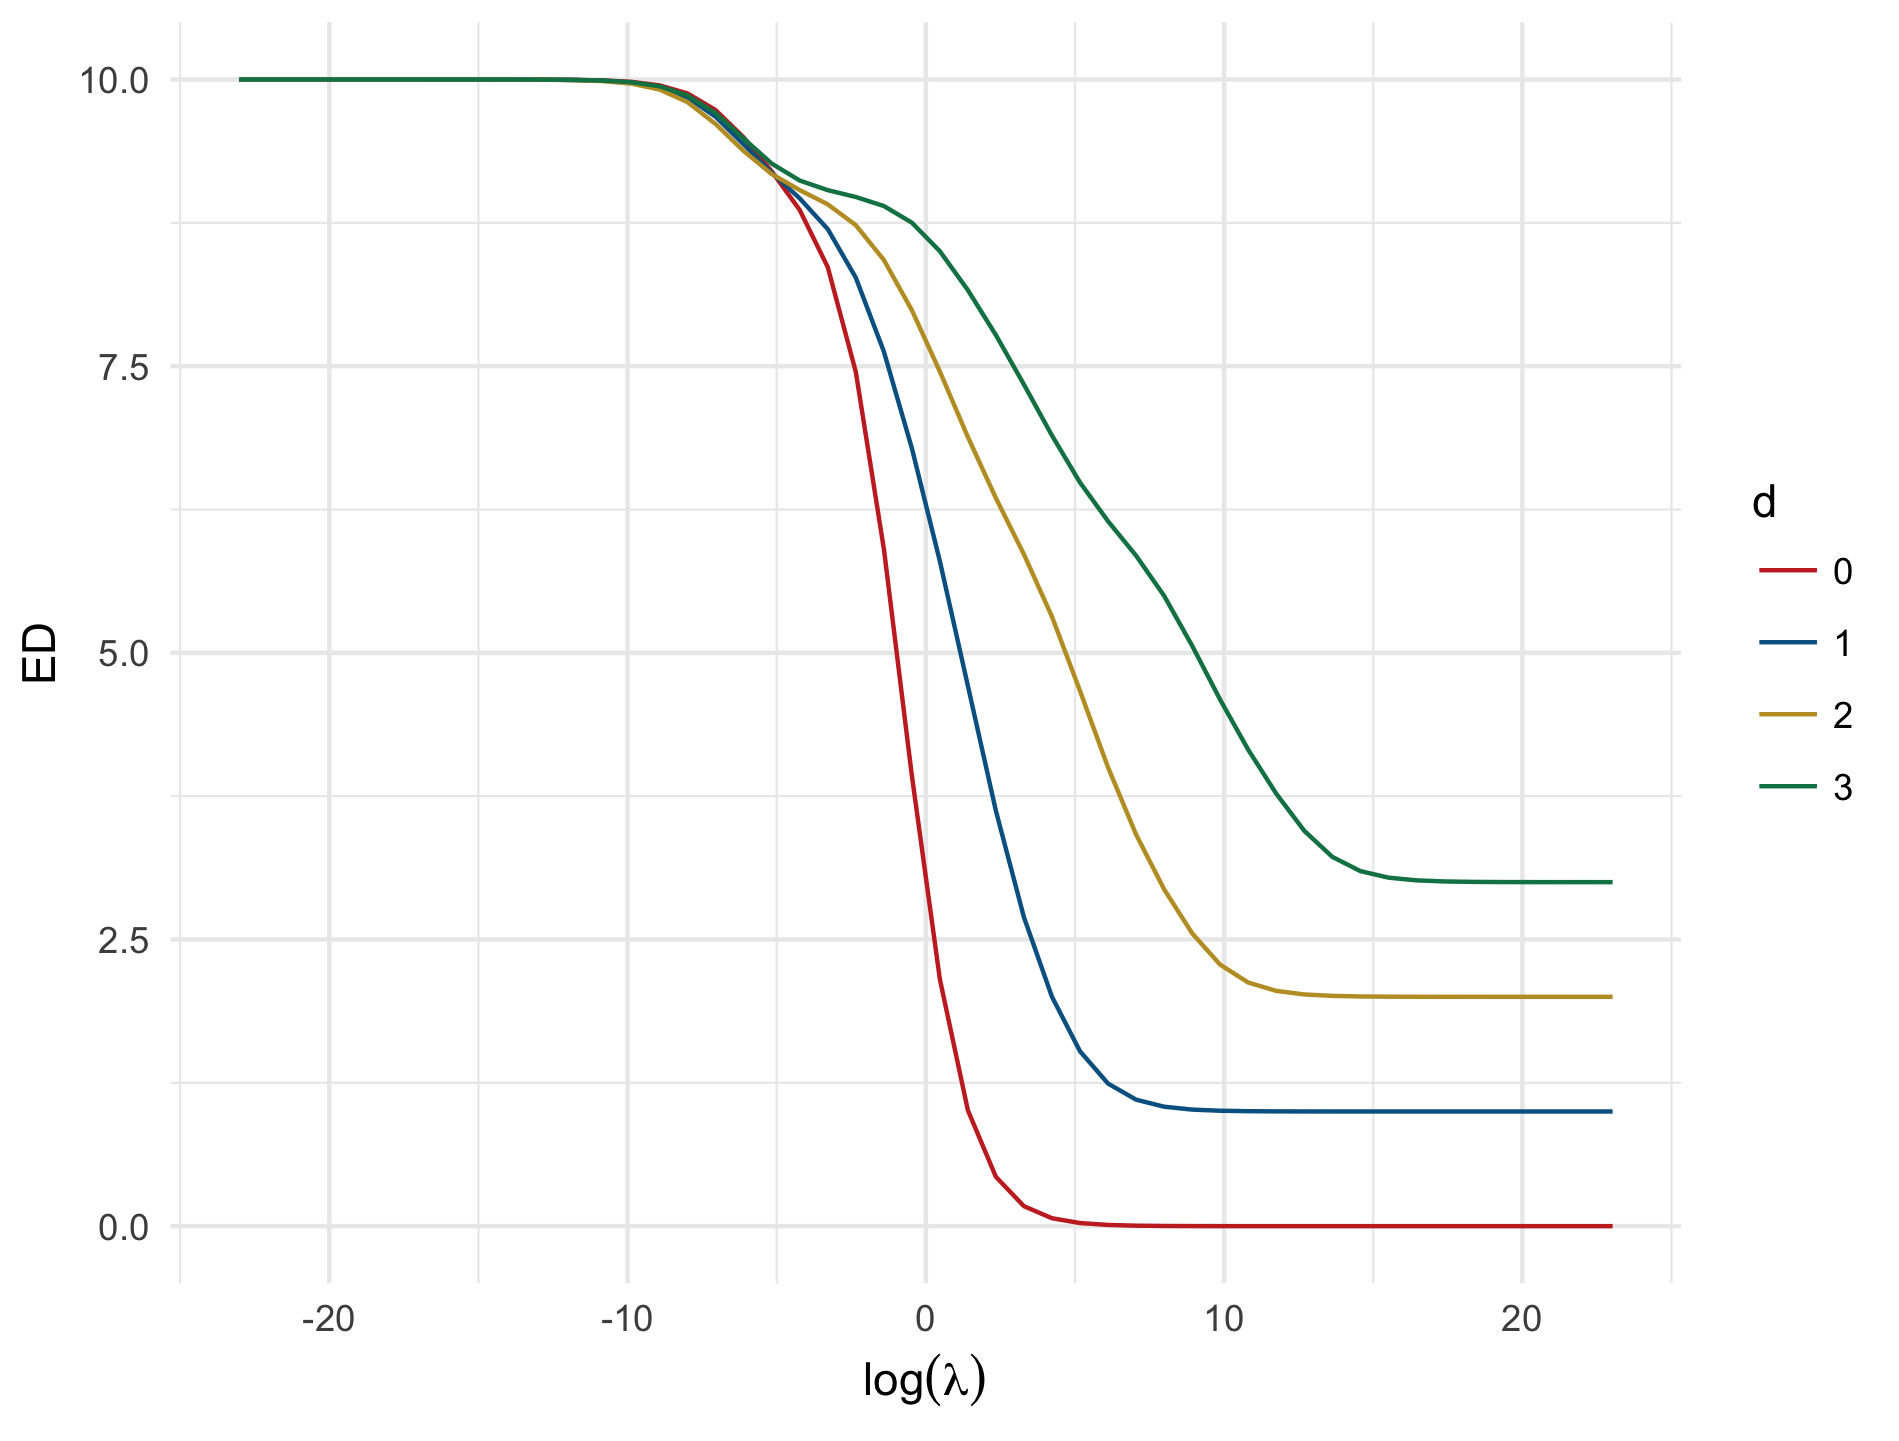
\includegraphics[width=0.7\textwidth]{pspline-limiting-effective-dimension}
%\caption{\textit{The limiting behaviour of the trace of the smoothing matrix $A_\lambda$ as the smoothing parameter increases for the P-spline fit to the 10 observations using 60 B-spline basis functions, shown in Figure~\ref{fig:overcomplete-pspline-basis}. For weakly enforced smoothing, the effective dimension is equal to the number of observations, and as $\lambda \rightarrow \infty$, the effective dimension approaches the order of the difference penalty.}} \label{fig:pspline-limiting-effective-dimension}
%\end{center}
%\end{figure}
%
%The effective model dimension is closely connected to model selection criteria; \cite{eilers1996flexible} propose the use of the Akaike information criterion (AIC) for selecting the optimal value of the smoothing parameters $\lambda = \left(\lambda_l, \lambda_m\right)$, which is equivalent to the unbiased risk estimator discussed in Chapter~\ref{SSANOVA-chapter} under a Gaussian likelihood. For a detailed discussion of the connection between the unbiased risk estimate and AIC in the non-gaussian case, see \cite{wood2017generalized}, Chapter 4, Section 5. The same reference provides a detailed discussion of computational methods for minimizing the unbiased risk estimate with respect to multiple smoothing parameters. The algorithm shares the same basic structure as the one outlined in Section~\ref{gaussian-unbiased-risk-estimate}, with modifications on the derivatives and the Hessians to account for the fact that the P-spline basis and penalty are constructed independently of one another.
%


\section{The P-spline Estimator for the Innovation Variance Function}

The P-spline estimator for the log innovation variance function is constructed via penalized similarly to the smoothing spline estimator in Section~\ref{chapter-3-IV-modeling-section}.  Fixing $\phi = \phi^*$ at an estimate $\phi^*$ of $\phi$, the the log likelihood of the squared working residuals can be written as in \eqref{eq:penalized-joint-loglik-given-phi-2}
\[
-2\ell\left( \sigma^2  \vert Z_1,\dots, Z_N, \phi,  \right) =  \sum_{i = 1}^N \sum_{j = 1}^{p_i} \log \sigma^2_{ij}  + \sum_{i = 1}^N \sum_{j = 1}^{p_i} \frac {z_{ij}}{\sigma^2_{ij}},
\]
\noindent
where $\epsilon_{ij} =  y_{ij} - \sum\limits_{k<j} \phi^*_{ijk} y_{ik}$, and $z_{ij} = \epsilon_{ij}^2$. We can approximate $\eta \left(t\right) = \log \sigma^2\left(t\right)$ using a B-spline basis expansion, letting
\[
\eta\left(t\right) = \sum\limits_{j = 1}^{k_t} \theta_j B_{j}\left(t\right).
\] 
\noindent
Model estimation and smoothing parameter selection can be carried out using performance-oriented iteration as described in Section~\ref{smoothing-parameter-selection-exponential-families}, substituting the above expansion for $\eta$ and trading the smoothing spline penalty for the discrete difference penalty \eqref{eq:bspline-difference-penalty-1}. For detailed presentation of optimization procedures, see \cite{marx1999generalized}. 

